% (c) 2012 Tiziana Manca - tmanca@libero.it
% (c) 2012 - 2014 Dimitrios Vrettos - d.vrettos@gmail.com

\chapter{Relazioni}
%===================================
\section{Proposizioni e predicati}
In matematica frasi come ``19 è maggiore di~5'' o ``Giove ruota intorno alla Terra'' sono considerate \emph{proposizioni} perché ad esse
si può attribuire un preciso valore di verità, cioè si può stabilire se sono vere oppure false: la prima è una proposizione vera, la seconda è falsa.

Non sono proposizioni in senso matematico ``Cosa stai studiando?'', ``domani pioverà!'', ``$x$ è un numero primo'':
infatti la prima non è un'affermazione ma pone una domanda, la seconda è una esclamazione e quindi non possiamo stabilire se è vera o falsa;
l'ultima contiene un elemento indeterminato e finché non si fissa il valore da attribuire a~$x$, non si può decidere se la frase che lo riguarda è vera o falsa.

Ogni proposizione è formata da un \emph{predicato} (verbo) e dai suoi \emph{argomenti} (cose o persone alle quali il verbo si riferisce).

Analizzando le proposizioni sopra enunciate si ha:
\begin{center}
\begin{tabular}{llc}
\toprule
Soggetto & Predicato & Complemento \\
\midrule
19 & è maggiore di & 5 \\
Giove & ruota attorno alla & Terra \\
\bottomrule
\end{tabular}
\end{center}
Il soggetto e il complemento sono gli argomenti ai quali il predicato si riferisce.
In alcune proposizioni il predicato si riferisce a due argomenti (il \emph{soggetto} e il \emph{complemento})
in altre ad un solo argomento: ad esempio, il predicato ``essere numero primo'' stabilisce semplicemente una caratteristica del numero~5
senza porre alcuna connessione con un altro argomento.

\begin{definizione}\label{def:predicato_binario}
Si dice \emph{predicato binario} un predicato che si riferisce a due argomenti.
\end{definizione}

\ovalbox{\risolvi \ref{ese:7.1}}

\section{Relazioni in un insieme}

Il termine \emph{relazione} entra molto spesso in frasi del linguaggio naturale, lo usiamo per esprimere un generico legame tra due persone o tra due oggetti,
anche senza specificarne la natura: ``si è conclusa la relazione tra Anna e Paolo'', ``l'allungamento di una sbarretta di ferro è in relazione con il calore fornito'',
``la frana del terreno è in relazione con il disboscamento della zona e l'abusivismo edilizio'', ``domani consegnerò la relazione di fisica''.
Sono tutte espressioni che ci danno informazioni di un qualche collegamento tra gli
argomenti (persone, cose) ai quali il termine relazione si riferisce.

Dal punto di vista matematico diamo la seguente definizione.
\begin{definizione}
Si dice \emph{relazione} in un insieme~$A$ un predicato binario che lega due elementi dell'insieme.
\end{definizione}

\begin{exrig}
 \begin{esempio}
 Nell'insieme~$A = \{3\text{,~}5\text{,~}6\text{,~}9\text{,~}30\}$ è introdotto il predicato binario ``essere multiplo di''; con esso formiamo le proposizioni vere scegliendo soggetto e
 complemento nell'insieme~$A$:

\begin{multicols}{3}
30 è multiplo di~6;

9 è multiplo di~3;

%30 è multiplo di~3;

%6 è multiplo di~3;

30 è multiplo di~5;

3 è multiplo di~3;

%5 è multiplo di~5;

%6 è multiplo di~6;

9 è multiplo di~9;

\ldots
\end{multicols}
Il predicato ``essere multiplo'' genera nell'insieme~$A$ una relazione matematica. Esso non è il
solo che permette di collegare tra loro due elementi di quell'insieme.
\end{esempio}
\end{exrig}

\ovalbox{\risolvi \ref{ese:7.2}}\vspazio

Se chiamiamo con~$\Rel$ il predicato binario che definisce la relazione introdotta nell'insieme, per indicare 
sinteticamente la proposizione avente come soggetto~$a$, come complemento~$b$ e come predicato~$\Rel$, scriviamo~$a \,\Rel\, b$ e
diremo che~\emph{$a$ è in relazione con~$b$}.

\begin{exrig}
 \begin{esempio}

Con riferimento all'esempio precedente si ha:~$A = \{3\text{,~}5\text{,~}6\text{,~}9\text{,~}30\}$ e $\Rel$:
``essere multiplo di''. Allora scriviamo: per qualunque~$a$ e~$b$ appartenenti ad~$A$,
$a \,\Rel\, b$ se e solo se~$a$ è multiplo di~$b$, in simboli: $\forall a,b \in A \Leftrightarrow a \text{ è multiplo di } b$
\[30 \,\Rel\,~6;\quad~9 \,\Rel\,~3;\quad~30 \,\Rel\,~3;\quad~6 \,\Rel\,~3;\quad~30 \,\Rel\,~5;\quad~3 \,\Rel\,~3;\quad 5 \,\Rel\,~5;\quad~6 \,\Rel\,~6;\quad~9 \,\Rel\,~9;\quad~30 \,\Rel\,~30.\]

Abbiamo così formato un insieme di coppie ordinate di elementi tra loro in relazione:~$30 \,\Rel\,~5$ può anche essere indicata con la coppia ordinata~$(30;5)$.
\end{esempio}
\end{exrig}

\begin{definizione}
Chiamiamo \emph{insieme della relazione} $G_\Rel$ l'insieme delle coppie ordinate i cui
elementi sono gli argomenti del predicato binario, ossia sono in relazione tra di loro. Esso risulta essere un
sottoinsieme del prodotto cartesiano dell'insieme~$A$ con se stesso. Si rappresenta per proprietà caratteristica nel
seguente modo~$G_\Rel = \{(a;b) \in A \times A \mid  a \,\Rel\, b \}$.
\end{definizione}

\ovalbox{\risolvii \ref{ese:7.3}, \ref{ese:7.4}, \ref{ese:7.5}, \ref{ese:7.6}}
%===================================
\subsection{Grafico di una relazione}

Dal momento che una relazione in un insieme~$Y$ determina un sottoinsieme del prodotto cartesiano~$Y \times Y$, è
comodo rappresentare una relazione nello stesso diagramma usato per rappresentare il prodotto cartesiano.
Una relazione può quindi essere rappresentata attraverso un \emph{grafico cartesiano}.

\ovalbox{\risolvii \ref{ese:7.7}, \ref{ese:7.8}}

%===================================
\subsection{Matrice o tabella di una relazione}

Nella figura~\ref{fig:7.1} è rappresentata la classica griglia per il gioco della battaglia navale.
Ogni cella è individuata da una coppia ordinata il cui primo elemento (una lettera dell'alfabeto) indica la riga,
il secondo (un numero) indica la colonna; così la coppia~$(D;5)$ indica la cella annerita.

\ovalbox{\risolvii \ref{ese:7.9}, \ref{ese:7.10}, \ref{ese:7.11}}

%===================================
\subsection{Grafo di una relazione}

\begin{definizione}
Un \emph{grafo} è un insieme di punti, detti \emph{nodi}, e di archi che uniscono coppie di punti.
\end{definizione}

%Abbiamo visto che con un predicato si possono formare alcune proposizioni aventi rispettivamente come soggetto e
%come complemento elementi di un insieme: solo le proposizioni vere determinano la relazione tra gli elementi di
%quell'insieme e generano coppie di elementi in relazione.

\begin{exrig}
 \begin{esempio}

Nel diagramma di Eulero-Venn di figura~\ref{fig:7.2}, relativo all'insieme~$A = \{$3, 5, 6, 9, 30$\}$
rappresentiamo la relazione~$\Rel$ = ``essere multiplo di'' collegando, mediante una freccia, gli argomenti delle proposizione vere.

Come puoi osservare, l'elemento~30 è collegato con una freccia all'elemento~6 in quanto la proposizione ``30 è multiplo di~6'' è vera, ma non all'elemento~9
poiché la proposizione ``30 è multiplo di~9'' è falsa; inoltre la punta della freccia è sul numero~6 in quanto complemento del predicato ``essere multiplo di'' (si parla in tal caso di \emph{grafo orientato});
infine su ciascun elemento abbiamo messo un ``anello'' o ``cappio'' per indicare che ogni elemento è in relazione con se stesso visto che per ogni
elemento~$a \in A$ la proposizione ``$a$ è multiplo di~$a$'' risulta vera.

 \end{esempio}
\end{exrig}

\ovalbox{\risolvii \ref{ese:7.12}, \ref{ese:7.13}, \ref{ese:7.14}, \ref{ese:7.15}, \ref{ese:7.16}, \ref{ese:7.17}}
\begin{figure}[hb]
\begin{minipage}[t]{.45\textwidth}
 \centering
 % (c) 2012 Dimitrios Vrettos - d.vrettos@gmail.com

\begin{tikzpicture}[x=10mm,y=10mm, font=\small,table nodes/.style={%
		rectangle,
		draw=black,
 		align=center,
   		minimum height=5mm,
     	text depth=0.5ex,
     	text height=1.5ex,
     	inner xsep=-1pt,
     	outer sep=0pt
	},
	table/.style={%
        matrix of nodes,
        row sep=-\pgflinewidth,
        column sep=-\pgflinewidth,
        nodes={%
            table nodes
        },
        execute at empty cell={\node[fill=black]{};}
    }]

\matrix (first) [table,text width=7mm,name=table]
{
{}  & 1 & 2 & 3 &4 & 5 & 6 & 7\\
$A$ &{} &{} &{} &{} &{} &{} &{} \\
$B$ &{} &{} &{} &{} &{} &{} &{} \\
$C$ &{} &{} &{} &{} &{} &{} &{} \\
$D$ &{} &{} &{} &{} & &{} &{}  \\
$E$ &{} &{} &{} &{} &{} &{} &{} \\
$F$ &{} &{} &{} &{} &{} &{} &{} \\
};

\end{tikzpicture}

 \caption{Griglia della battaglia navale.}\label{fig:7.1}
\end{minipage}\hfil
\begin{minipage}[t]{.45\textwidth}
 \centering
 % (c) 2012 Dimitrios Vrettos - d.vrettos@gmail.com

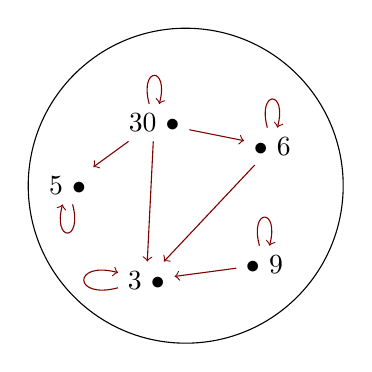
\begin{tikzpicture}[x=10mm,y=10mm, every state/.style={draw=CornflowerBlue}, every loop/.style={draw=Maroon}]
\draw (0,0) circle (2);

\node (5) at (-1.5,0) {$5~ \bullet$};
\node (30) at (-.4,.8) {$30~\bullet$};
\node(6) at (1.1,.5) {$\bullet~6$};
\node (9) at (1,-1) {$\bullet~9$};
\node (3) at (-.5,-1.2) {$3~\bullet$};

\begin{scope}[->]
\path(5) edge[loop below] node{} ()
	(30) edge[loop above] node{} ()
	(6) edge[loop above] node{} ()
	(9) edge[loop above] node{} ()
	(3) edge[loop left] node{} ();

\end{scope}
\begin{scope}[->, Maroon]
\draw (30)--(5);
\draw (30)--(6);
\draw (30)--(3);
\draw (6)--(3);
\draw (9)--(3);
\end{scope}
\end{tikzpicture}

 \caption{L'insieme~$A$.}\label{fig:7.2}
\end{minipage}
\end{figure}

\pagebreak
\section{Proprietà delle relazioni}
%===================================
\subsection{Proprietà riflessiva}

\begin{exrig}
 \begin{esempio}

Nell'insieme~$T = \{\text{4, 7, 8, 12, 35, 100}\}$ è introdotta la relazione~$\Rel$: ``essere divisore di''.
Puoi verificare che ogni numero è divisore di se stesso, cioè ogni elemento dell'insieme è in relazione
con se stesso. Una relazione di questo tipo si dice che gode della \emph{proprietà riflessiva}.
Osserva, però, che nell'insieme ~$\insN$ dei numeri naturali la relazione ``essere divisibile per'' non è riflessiva poiché zero non è divisibile per se stesso.
 \end{esempio}
\end{exrig}

\begin{definizione}
Una relazione~$\Rel$ in un insieme~$A$ gode della \emph{proprietà riflessiva} quando ogni elemento è in relazione con se stesso, ossia per qualunque~$x$ dell'insieme~$A$ si ha~$x \,\Rel\, x$.
In simboli: $\forall x \in A: x \,\Rel\, x$.
\end{definizione}

\ovalbox{\risolvi \ref{ese:7.18}}

%===================================
\subsection{Proprietà antiriflessiva}

\begin{exrig}
 \begin{esempio}
Nell'insieme delle persone~$P = \{\text{Marco, Antonio, Carlo}\}$ è data la relazione~$\Rel$: ``essere più alto di''. Nessun elemento è in relazione con se stesso, infatti nessuno può essere più alto di se stesso.
 \end{esempio}
\end{exrig}

\begin{definizione}
Una relazione~$\Rel$ in un insieme~$A$ gode della \emph{proprietà antiriflessiva} quando nessun elemento è in relazione con se stesso,
ossia per nessun elemento~$x$ di~$A$ si ha~$x \,\Rel\, x$.
In simboli: $\nexists x \in A:\, x \,\Rel\, x$.
\end{definizione}

\ovalbox{\risolvi \ref{ese:7.19}}
\subsection{Proprietà simmetrica}

\begin{exrig}
 \begin{esempio}
Nella relazione~$\Rel$: ``essere concorde con'' nell'insieme dei numeri~$A = \{-1\text{, }+3\text{, }-7\text{, }+5\text{, }-2\text{, }+4\text{, }+10\}$ si può osservare che se un elemento dell'insieme è in relazione con un altro allora anche quest'ultimo è in relazione con il primo:
$-1 \,\Rel\, -7$, ma anche~$-7 \,\Rel\, -1$; $+3 \,\Rel\, +5$, ma anche~$+5 \,\Rel\, +3$ e così via.
 \end{esempio}
\end{exrig}

%\begin{figure}[ht]
%\begin{minipage}[t]{.45\textwidth}
% \centering
% % (c) 2012 Dimitrios Vrettos - d.vrettos@gmail.com

\begin{tikzpicture}[x=10mm,y=10mm, font=\small, every state/.style={draw=CornflowerBlue}, every loop/.style={draw=Maroon}]
\draw (0,0) circle (1.8);

\node at (1.8,1.5) {$P$};

\node[state] (M) at (-1,.3) {$M$};
\node[state] (C) at (.8,.8) {$C$};
\node[state] (A) at (.2,-1) {$A$};

 \begin{scope}[->, Maroon]
 \draw (M)--(C);
 \draw (M)--(A);
 \draw (C)--(A);
 \end{scope}
\end{tikzpicture}
% \caption{Proprietà antiriflessiva.}\label{fig:B.3}
%\end{minipage}\hfil
%\begin{minipage}[t]{.45\textwidth}
% \centering
% % (c) 2012 Dimitrios Vrettos - d.vrettos@gmail.com

\begin{tikzpicture}[x=10mm,y=10mm, font=\small, every state/.style={draw=CornflowerBlue}, every loop/.style={draw=Maroon}]
\draw (0,0) circle [x radius=3, y radius=2];

\node[state] (A) at (-2.3,.3) {$-1$};
\node[state] (B) at (-.8,1.2) {$-2$};
\node[state] (C) at (-1.5,-1) {$-7$};
\node[state] (D) at (-.5,-.9) {$+10$};
\node[state] (E) at (.6,.9) {$+3$};
\node[state] (F) at (1.8,.5) {$+4$};
\node[state] (G) at (1.5,-1) {$+5$};

\begin{scope}[->]
\path(A) edge[loop below] node{} ()
	(B) edge[loop right] node{} ()
	(C) edge[loop left] node{} ()	
(D) edge[loop below] node{} ()
	(E) edge[loop above] node{} ()
	(F) edge[loop right] node{} ()
	(G) edge[loop right] node{} ();

\end{scope}
% \begin{scope}[<->, Maroon]
 \begin{scope}[-, Maroon]
 \draw (A)--(C);
 \draw (B)--(A);
 \draw (C)--(B);
\draw (D)--(E);
\draw (D)--(F);
\draw (E)--(F);
\draw (G)--(F);
\draw (E)--(G);
\draw (D)--(G);
 \end{scope}
\end{tikzpicture}

% \caption{Proprietà simmetrica.}\label{fig:B.4}
%\end{minipage}
%\end{figure}

\begin{definizione}
Una relazione~$\Rel$ in un insieme~$A$ gode della \emph{proprietà simmetrica} quando risultano vere le due proposizioni
che si ottengono scambiando soggetto e complemento; ossia per qualunque~$x$ e~$y$ appartenenti all'insieme~$A$ se vale~$x \,\Rel\, y$ allora vale anche~$y \,\Rel\, x$.
In simboli: $\forall x, y \in A:\, x \,\Rel\, y \rightarrow \, y \,\Rel\, x$
\end{definizione}

\ovalbox{\risolvi \ref{ese:7.20}}

%===================================
\subsection{Proprietà antisimmetrica}

\begin{exrig}
 \begin{esempio}

Il diagramma di Venn nella figura~\ref{fig:7.3} rappresenta un insieme~$U$ e alcuni suoi sottoinsiemi.

Consideriamo ora l'insieme di insiemi~$S = \{U\text{,~}A\text{,~}B\text{,~}C\text{,~}D\text{,~}E\text{,~}F\}$ e la relazione~$\Rel$: ``essere sottoinsieme proprio di''.
Completa il grafo della relazione.

Certamente nel completare il grafo (figura~\ref{fig:7.4}) non avrai usato archi poiché è evidente che le proposizioni ``$B$ è sottoinsieme proprio di~$C$'' e ``$C$
è sottoinsieme proprio di~$B$'' non possono essere entrambe vere. Anzi, la verità della prima implica necessariamente la falsità della seconda.
 \end{esempio}
\end{exrig}

\begin{figure}[hb]
\begin{minipage}[b]{.45\textwidth}
 \centering
 % (c) 2012 Dimitrios Vrettos - d.vrettos@gmail.com

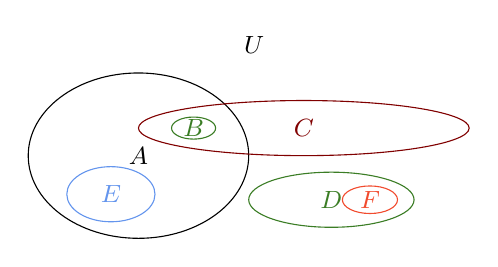
\begin{tikzpicture}[scale=.7,x=10mm,y=10mm, font=\small, every state/.style={draw=CornflowerBlue}, every loop/.style={draw=Maroon}]
\draw (0,0) circle [x radius=2, y radius=1.5] node {$A$};
\draw[CornflowerBlue] (-.5,-.7) circle [x radius=.8, y radius=.5]node {$E$};
\draw[OliveGreen] (1,.5) circle [x radius=.4, y radius=.2]node {$B$};
\draw[Maroon] (3,.5) circle [x radius=3, y radius=.5]node {$C$};
\draw[OliveGreen] (3.5,-.8) circle [x radius=1.5, y radius=.5]node {$D$};
\draw[RedOrange] (4.2,-.8) circle [x radius=.5, y radius=.25]node {$F$};

\node () at (2.1,2) {$U$};
\end{tikzpicture}
 \caption{L'insieme~$U$.}\label{fig:7.3}
\end{minipage}\hfil
\begin{minipage}[b]{.45\textwidth}
 \centering
 % (c) 2012 Dimitrios Vrettos - d.vrettos@gmail.com

\begin{tikzpicture}[scale=.7,x=10mm,y=10mm, font=\small, every state/.style={draw=CornflowerBlue}, every loop/.style={draw=Maroon}]
\draw (0,0) circle [x radius=3, y radius=2];

\node at (3,1.5) {$S$};
\node[state] (A) at (-2.3,.3) {$A$};
\node[state] (B) at (-.8,1.2) {$B$};
\node[state] (C) at (-1.5,-1) {$C$};
\node[state] (D) at (-.2,-1.1) {$D$};
\node[state] (E) at (.6,.9) {$E$};
\node[state] (F) at (1.8,.5) {$F$};
\node[state] (U) at (1.5,-1) {$U$};

  \begin{scope}[->, Maroon]
 \draw (A)--(U);
  \draw (B)--(C);
 \draw (F)--(U);
   \end{scope}
\end{tikzpicture}
 \caption{L'insieme~$S$.}\label{fig:7.4}
\end{minipage}
\end{figure}

\begin{definizione}
Una relazione~$\Rel$ in un insieme~$A$ gode della \emph{proprietà antisimmetrica} quando non possono essere vere
contemporaneamente le proposizioni che si ottengono scambiando il soggetto con il complemento, se soggetto e complemento sono diversi
tra loro; ossia per qualunque~$x$ e~$y$ dell'insieme~$A$ se~$x \neq y$ e se~$x \,\Rel\, y$ non è vero che~$y \,\Rel\, x$.
\end{definizione}

\ovalbox{\risolvi \ref{ese:7.21}}

%===================================
\subsection{Proprietà transitiva}
%
%\begin{exrig}
% \begin{esempio}
%
%Nel grafo di figura~\ref{fig:B.7} è rappresentata una relazione~$\Rel$ introdotta in un insieme~$T$. Dall'analisi della situazione rappresentata possiamo
%affermare che dalla verità di $a \,\Rel\, b$ e~$b \,\Rel\, c$ segue la verità di~$a \,\Rel\, c$. Analizzando gli altri elementi, 
%possiamo osservare che essendo vere $e \,\Rel\, f$ e~$f\, \Rel\, g$ è vera anche~$e \,\Rel\, g$;
%inoltre si ha che essendo vera $n \,\Rel\, m$ e~$m \,\Rel\, t$ è vera anche~$n \,\Rel\, t$.
% \end{esempio}
%\end{exrig}
%
%\begin{figure}[ht]
%\begin{minipage}[b]{.45\textwidth}
% \centering
% % (c) 2012 Dimitrios Vrettos - d.vrettos@gmail.com

\begin{tikzpicture}[x=10mm,y=10mm, font=\small, every state/.style={draw=CornflowerBlue}, every loop/.style={draw=Maroon}]
\draw (0,0) circle [x radius=3, y radius=2];

\node at (3,1.5) {$T$};
\node[state] (A) at (-2.3,.3) {$a$};
\node[state] (B) at (-.8,1.2) {$b$};
\node[state] (C) at (-1,0) {$c$};
\node[state] (G) at (.2,0) {$g$};
\node[state] (E) at (.6,1.3) {$e$};
\node[state] (F) at (1.8,.8) {$f$};
\node[state] (M) at (1.5,-1.1) {$m$};
\node[state] (N) at (0,-1.2) {$n$};
\node[state] (T) at (2.2,-.2) {$t$};
\begin{scope}[->, Maroon]
\draw (A)--(C);
\draw (B)--(C);
\draw (A)--(B);

\draw (E)--(F);
\draw (E)--(G);
\draw (F)--(G);

\draw (N)--(M);
\draw (N)--(T);
\draw (M)--(T);
\end{scope}
\end{tikzpicture}
% \caption{L'insieme~$T$.}\label{fig:B.7}
%\end{minipage}\hfil
%\begin{minipage}[b]{.45\textwidth}
% \centering
% % (c) 2012 Dimitrios Vrettos - d.vrettos@gmail.com

\begin{tikzpicture}[x=10mm,y=10mm, font=\small, every state/.style={draw=CornflowerBlue}, every loop/.style={draw=Maroon}]
\draw (0,0) circle [x radius=3, y radius=2];

\node at (3,1.5) {$B$};
\node[state] (A) at (-2.3,.3) {$a$};
\node[state] (H) at (-.8,1.2) {$h$};
\node[state] (F) at (-1.5,-1) {$f$};
\node[state] (B) at (-.5,-.3) {$b$};
\node[state] (E) at (.6,.9) {$e$};
\node[state] (C) at (1.8,.5) {$c$};
\node[state] (D) at (1.5,-.5) {$d$};
\node[state] (G) at (.5,-1.3) {$g$};
\begin{scope}[->]
\path(A) edge[loop below] node{} ()
(H) edge[loop right] node{} ()
(F) edge[loop left] node{} ()	
(B) edge[loop below] node{} ()
(E) edge[loop above] node{} ()
(C) edge[loop right] node{} ()
(D) edge[loop right] node{} ()
(G) edge[loop above] node{} ();
\end{scope}
\begin{scope}[-, Maroon]
\draw (A)--(H);
\draw (F)--(A);
\draw (F)--(H);
\draw (B)--(E);
\draw (B)--(C);
\draw (E)--(C);
\draw (G)--(D);
\end{scope}
\end{tikzpicture}
% \caption{L'insieme~$B$.}\label{fig:B.8}
%\end{minipage}
%\end{figure}

\begin{definizione}
Una relazione~$\Rel$ in un insieme~$A$ gode della \emph{proprietà transitiva} quando se~$a \,\Rel\, b$ e~$b \,\Rel\, c$
allora risulta anche~$a \,\Rel\, c$, con~$a$, $b$, $c$ elementi qualsiasi dell'insieme~$A$.
In simboli $\forall a, b, c \in A:\, a\, \Rel\, b\, \wedge\, a\,\Rel\,c\,\rightarrow\,a\,\Rel\,c$.
\end{definizione}

\ovalbox{\risolvii \ref{ese:7.22}, \ref{ese:7.23}, \ref{ese:7.24}, \ref{ese:7.25}}
\pagebreak
%===================================
\section{Relazioni di equivalenza}

\begin{exrig}
 \begin{esempio}

Completa la seguente tabella segnando le proprietà di cui gode (R=riflessiva, S=simmetrica, T=transitiva, AS=antisimmetrica, AR=antiriflessiva) ciascuna relazione.

\begin{center}
\begin{tabular}{lcc}
\toprule
Relazione & Insieme & Proprietà \\
\midrule
Avere lo stesso perimetro & poligoni & [R] \, [S]\, [T]\, [AS]\, [AR] \\
Essere fratello di & persone & [R] \, [S]\, [T]\, [AS]\, [AR] \\
Essere figlio di & persone & [R] \, [S]\, [T]\, [AS]\, [AR] \\
Essere più alto di & persone & [R] \, [S]\, [T]\, [AS]\, [AR] \\
Avere gli angoli rispettivamente congruenti & triangoli & [R] \, [S]\, [T]\, [AS]\, [AR] \\
Iniziare con la stessa lettera & parole & [R] \, [S]\, [T]\, [AS]\, [AR] \\
Giocare nella stessa squadra & calciatori & [R] \, [S]\, [T]\, [AS]\, [AR] \\
$a \,\Rel\, b$ se e solo se~$a$ è nato nello stesso anno di $b$ & persone & [R] \, [S]\, [T]\, [AS]\, [AR] \\
$x \,\Rel\, y$ se e solo se~$x$ ha lo stesso numero di cifre di $y$ & $\insN \times \insN $ &[R] \, [S]\, [T]\, [AS]\, [AR] \\
$x \,\Rel\, y$ se e solo se~$x$ ha la stessa ultima cifra di $y$ & $\insN \times \insN $ &[R] \, [S]\, [T]\, [AS]\, [AR] \\
%$x \,\Rel\, y$ se e solo se la somma delle cifre di~$x$ è maggiore quella di~$y$ & $\insN \times \insN $ &\boxR\quad\boxS\quad\boxT\quad\boxAS \\
$x \,\Rel\, y$ se e solo se~$x$ è multiplo di~$y$ & $\insN \times \insN $ &[R] \, [S]\, [T]\, [AS]\, [AR] \\
$x \,\Rel\, y$ se e solo se~$x+y$ è pari & $\insN \times \insN $ &[R] \, [S]\, [T]\, [AS]\, [AR] \\
Avere lo stesso segno zodiacale & persone & [R] \, [S]\, [T]\, [AS]\, [AR] \\
$(a;b) \,\Rel\, (x;y)$ se e solo se~$a+b=x+y$ & ~$\insN \times \insN$ & [R] \, [S]\, [T]\, [AS]\, [AR] \\
\bottomrule
\end{tabular}
\end{center}

\emph{Svolgimento}: La prima relazione gode delle tre proprietà riflessiva, simmetrica e transitiva; infatti:

\begin{itemize*}
\item ``il poligono~$P$ ha lo stesso perimetro di se stesso'' è vera per qualunque poligono (\emph{proprietà riflessiva});
\item ``il poligono~$P_1$ ha lo stesso perimetro del poligono~$P_2$'' implica la verità della proposizione ``il
poligono~$P_2$ ha lo stesso perimetro di~$P_1$'', qualunque siano i due poligoni~$P_1$ e~$P_2$ (\emph{proprietà
simmetrica});
\item se ``il poligono~$P_1$ ha lo stesso perimetro di~$P_2$'' e ``$P_2$ ha lo stesso perimetro di~$P_3$'' allora si ha anche che ``$P_1$ ha lo stesso
perimetro di~$P_3$'', qualunque siano i poligoni~$P_1$, $P_2$, $P_3$ (\emph{proprietà transitiva}).
\end{itemize*}

Verifica tu se anche le altre relazioni godono delle tre proprietà riflessiva, simmetrica, transitiva, come
``essere fratello di'', ``avere gli angoli rispettivamente uguali'', ``iniziare con la stessa lettera''.
 \end{esempio}
\end{exrig}

\begin{definizione}
Chiamiamo \emph{relazione d'equivalenza} una relazione che gode delle tre proprietà riflessiva, simmetrica e transitiva.
\end{definizione}

\ovalbox{\risolvi \ref{ese:7.26}}

\pagebreak

Premettiamo le definizioni:

\begin{definizione}
Dato un insieme $A$, suddividiamolo in un numero di sottoinsiemi~$A_1$, $A_2$, \ldots, $A_n$, detti \emph{classi}, tali che
\begin{enumeratea}
\item nessun sottoinsieme è vuoto;
\item a due a due sono disgiunti (non hanno tra loro alcun elemento in comune);
\item la loro unione è l'insieme~$A$.
\end{enumeratea}
L'insieme $P(A) = \{A_1$, $A_2$, \ldots, $A_n\}$ è detto \emph{partizione} di~$A$.
\end{definizione}

\begin{definizione}
In un insieme~$A$ dove sia stata definita una relazione d'equivalenza $\Rel$, si chiama \emph{classe d'equivalenza} ogni sottoinsieme di~$A$ contenente tutti e soli gli elementi
tra loro in relazione secondo $\Rel$.
\end{definizione}

Si viene così a determinare una partizione dell'insieme~$A$ in classi d'equivalenza, ognuna delle quali è indicata racchiudendo tra parentesi quadrate
uno degli elementi della classe considerata.

\begin{definizione}
Si chiama \emph{insieme quoziente} di un insieme~$A$ rispetto alla relazione di equivalenza~$\Rel$ in esso definita,
l'insieme i cui elementi sono le classi d'equivalenza determinate dalla relazione~$\Rel$, ovvero la partizione di~$A$ definita da~$\Rel$. L'insieme quoziente si indica con il simbolo~$A/\Rel$.
\end{definizione}

\osservazione Ogni volta che si ha una relazione d'equivalenza~$\Rel$ in un insieme~$A$, possiamo stabilire la seguente
catena di passaggi:
 \[\text{insieme }A\rightarrow\Rel\rightarrow\text{ partizione }\wp(A)=\text{ insieme quoziente }A/\Rel.\]

\begin{exrig}
 \begin{esempio}
Nell'insieme~$A = \{x \in \insN \mid 0\le x\le 20\}$ è data la relazione $\Rel=$ ``avere lo stesso resto nella divisione per~5''.
Vediamo alcuni numeri che sono in relazione:
\begin{multicols}{2}
0 : 5 \, quoziente~0 \, resto~0;

1 : 5 \, quoziente~0 \, resto~1;

2 : 5 \, quoziente~0 \, resto~2;

3 : 5 \, quoziente~0 \, resto~3;

4 : 5 \, quoziente~0 \, resto~4;

5 : 5 \, quoziente~1 \, resto~0;

6 : 5 \, quoziente~1 \, resto~1;

7 : 5 \, quoziente~1 \, resto~2;

8 : 5 \, quoziente~1 \, resto~3;

9 : 5 \, quoziente~1 \, resto~4;

10 : 5 \, quoziente~2 \, resto~0;

11 : 5 \, quoziente~2 \, resto~1;

12 : 5 \, quoziente~2 \, resto~2;

\ldots \ldots
\end{multicols}
Sono quindi in relazione:
\begin{itemize*}
\item $0 \, \Rel \,5$, $5 \, \Rel \,10$, $10 \, \Rel \,15$,  $15 \, \Rel \,20 \ldots$;
\item $1 \, \Rel \,6$, $6 \, \Rel \,11$, $11 \, \Rel \,16$,  $21 \, \Rel \,26 \ldots$;
\item $2 \, \Rel \,7$, $7 \, \Rel \,12$, $12 \, \Rel \,17$,  $27 \, \Rel \,32 \ldots$
\item $\ldots\ldots\ldots\ldots\ldots$
\end{itemize*}

Vediamo quali proprietà verifica la relazione~$\Rel$:
\begin{itemize*}
\item \emph{Riflessiva}: perché ogni numero ha lo stesso resto di se stesso nella divisione per~5. $0 \, \Rel 0$, $1 \, \Rel 1$, $2 \, \Rel 2$, \ldots;
\item \emph{Simmetrica}: Se $m \,\Rel \, n $ significa che ${resto}(m:5)={resto}(n:5)$ allora vale anche ${resto}(n:5)={resto}(m:5)$ e quindi $n \,\Rel \, m$;
\item \emph{Transitiva}: Se $m \,\Rel \, n $ e $n \,\Rel \, p $ significa che ${resto}(m:5)={resto}(n:5)={resto}(p:5)$ e quindi $m \,\Rel \, p$.
\end{itemize*}
Possiamo concludere che $\Rel$ è una relazione di equivalenza.

Rappresentiamo la partizione dell'insieme~$A$ secondo la relazione~$\Rel$.
\begin{center}
 % (c) 2015 Claudio Carboncini - claudio.carboncini@gmail.com
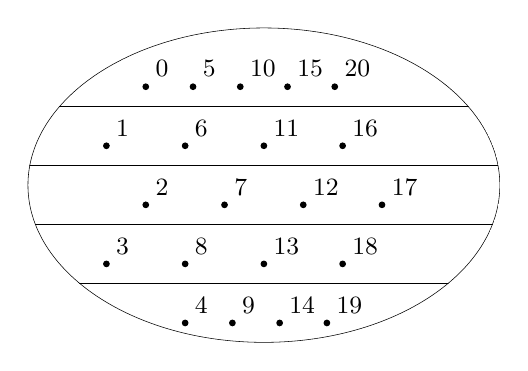
\begin{tikzpicture}[x=5mm, y=5mm,font=\small]

\clip (0,0) ellipse (6 and 4);

\draw (0,0) ellipse (6 and 4);

\draw[fill](-3,2.5) circle (1pt ) node[above right]  {0};
\draw[fill](-1.8,2.5) circle (1pt ) node[above right]  {5};
\draw[fill](-.6,2.5) circle (1pt ) node[above right]  {10};
\draw[fill](.6,2.5) circle (1pt ) node[above right]  {15};
\draw[fill](1.8,2.5) circle (1pt ) node[above right]  {20};

\draw(-6,2)--(6,2);

\draw[fill](-4,1) circle (1pt ) node[above right]  {1};
\draw[fill](-2,1) circle (1pt ) node[above right]  {6};
\draw[fill](0,1) circle (1pt ) node[above right]  {11};
\draw[fill](2,1) circle (1pt ) node[above right]  {16};

\draw(-6,.5)--(6,.5);

\draw[fill](-3,-.5) circle (1pt ) node[above right]  {2};
\draw[fill](-1,-.5) circle (1pt ) node[above right]  {7};
\draw[fill](1,-.5) circle (1pt ) node[above right]  {12};
\draw[fill](3,-.5) circle (1pt ) node[above right]  {17};

\draw(-6,-1)--(6,-1);

\draw[fill](-4,-2) circle (1pt ) node[above right]  {3};
\draw[fill](-2,-2) circle (1pt ) node[above right]  {8};
\draw[fill](0,-2) circle (1pt ) node[above right]  {13};
\draw[fill](2,-2) circle (1pt ) node[above right]  {18};

\draw(-6,-2.5)--(6,-2.5);

\draw[fill](-2,-3.5) circle (1pt ) node[above right]  {4};
\draw[fill](-.8,-3.5) circle (1pt ) node[above right]  {9};
\draw[fill](.4,-3.5) circle (1pt ) node[above right]  {14};
\draw[fill](1.6,-3.5) circle (1pt ) node[above right]  {19};

\end{tikzpicture}

\end{center}
Le classi di equivalenza sono:
\begin{itemize*}
\item $ [0]=\{0\text{, }5\text{, }10\text{, }15\text{, }20\} $;
\item $ [1]=\{1\text{, }6\text{, }11\text{, }16\} $;
\item $ [2]=\{2\text{, }7\text{, }12\text{, }17\} $;
\item $ [3]=\{3\text{, }8\text{, }13\text{, }18\} $;
\item $ [4]=\{4\text{, }9\text{, }14\text{, }19\} $.
\end{itemize*}
 \end{esempio}
\end{exrig}

\ovalbox{\risolvii \ref{ese:7.27}, \ref{ese:7.28}, \ref{ese:7.29}, \ref{ese:7.30}, \ref{ese:7.31}\ref{ese:7.32}, \ref{ese:7.33}, \ref{ese:7.34}, \ref{ese:7.35}, \ref{ese:7.36}, \ref{ese:7.37}}

\section{Relazioni di ordine}

Nel linguaggio di ogni giorno avrai certamente spesso usato espressioni come ``devo mettere in ordine i miei
libri'' oppure ``qui non c'è ordine'' e altre espressioni simili.
Anche in matematica, fin dalla scuola elementare, hai imparato a ordinare gli elementi dell'insieme dei
numeri naturali: dati due numeri naturali hai imparato infatti a stabilire quale dei due è il maggiore.

\begin{definizione}
Una relazione~$\Rel$, introdotta in un insieme~$A$, si chiama \emph{relazione d'ordine} se è antisimmetrica e transitiva.
\end{definizione}

Riguardando le varie relazioni introdotte sin qui, possiamo stabilire che esistono relazioni d'ordine di vario tipo, schematizzate nel seguente diagramma:
\begin{center}
 % (c) 2012 Dimitrios Vrettos - d.vrettos@gmail.com

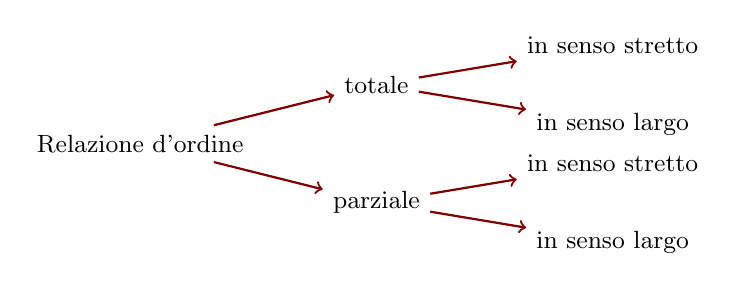
\begin{tikzpicture}[x=10mm,y=10mm, font=\small]

\node {Relazione d'ordine}[grow=right,level distance= 30mm, sibling distance=15mm,->,thick, draw=Maroon]
child {node {parziale}[sibling distance=10mm]
child {node {in senso largo}}
child {node {in senso stretto}}}
child {node {totale}[sibling distance=10mm]
child {node {in senso largo}}
child {node {in senso stretto}}};

\end{tikzpicture}

\end{center}

Attraverso alcuni esempi, vogliamo chiarire le differenze tra i diversi tipi. A questo scopo introduciamo la seguente definizione.

\begin{definizione}
Data una relazione d'ordine~$\Rel$ definita in un insieme~$A$, due elementi distinti~$x$ e~$y$ sono \emph{confrontabili} se rispetto a~$\Rel$ si ha~$x \,\Rel\, y$ oppure~$y \,\Rel\, x$.
\end{definizione}

\begin{definizione}
Una relazione d'ordine si dice \emph{parziale} quando esistono almeno due elementi che non sono confrontabili.
\end{definizione}

\begin{definizione}
Una relazione d'ordine si dice \emph{totale} quando due qualsiasi elementi possono essere messi in relazione, cioè sono confrontabili.
\end{definizione}

\begin{definizione}
Una relazione d'ordine è detta \emph{in senso largo} quando essa gode della proprietà riflessiva.
\end{definizione}

\begin{definizione}
Una relazione d'ordine è detta \emph{in senso stretto} quando essa gode della proprietà antiriflessiva.
\end{definizione}

\begin{center}
 % (c) 2012 Dimitrios Vrettos - d.vrettos@gmail.com

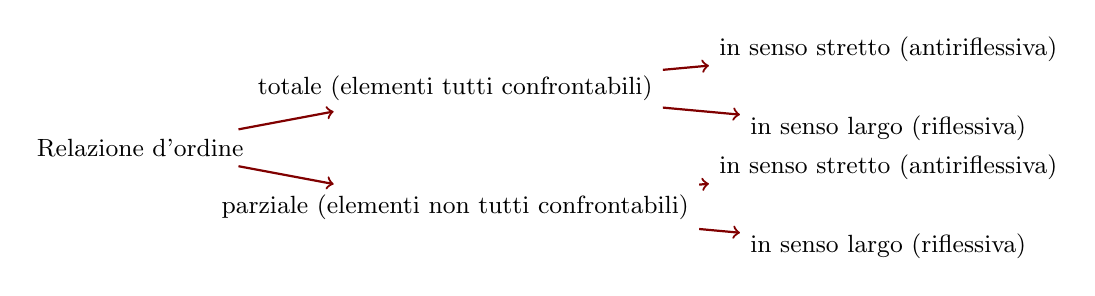
\begin{tikzpicture}[x=10mm,y=10mm, font=\small]

\node {Relazione d'ordine}[grow=right,level distance= 40mm,->,thick, draw=Maroon]
child {node {parziale (elementi non tutti confrontabili)}[level distance=55mm,sibling distance=10mm]
child {node {in senso largo (riflessiva)}}
child {node {in senso stretto (antiriflessiva)}}}
child {node {totale (elementi tutti confrontabili)}[level distance=55mm,sibling distance=10mm]
child {node {in senso largo (riflessiva)}}
child {node {in senso stretto (antiriflessiva)}}};

\end{tikzpicture}

\end{center}

\begin{exrig}
 \begin{esempio}
Nell'insieme degli alunni della tua classe considera la relazione $A \, \Rel \, B$ se il numero di lettere del nome di A è minore del numero di lettere del nome di B.
Verifichiamo le proprietà della relazione:
\begin{enumerate*}
\item \emph{Antiriflessiva}: perché ogni alunno non può avere un nome con meno lettere del suo nome;
\item \emph{Antisimmetrica}: se A ha il nome più corto del nome di B, non può accadere l'inverso e cioè che anche B abbia il nome più corto del nome di A;
\item \emph{Transitiva}: perché se A ha il nome più corto di~B e B ha il nome più corto di C allora anche $A \, \Rel \, C$.
\end{enumerate*}
Si tratta quindi di una \emph{relazione d'ordine parziale in senso stretto}. É parziale perché ci possono essere due alunni che avendo il nome con lo stesso numero di lettere non sono confrontabili nella relazione considerata.
 \end{esempio}
\end{exrig}

\ovalbox{\risolvii \ref{ese:7.38}, \ref{ese:7.39}, \ref{ese:7.40}, \ref{ese:7.41}, \ref{ese:7.42}, \ref{ese:7.43}}

\section{Relazioni tra due insiemi diversi}

Nei paragrafi precedenti abbiamo analizzato relazioni con predicato binario che si riferisce a due elementi dello stesso insieme, consideriamo ora relazioni con predicato binario in cui soggetto e complemento appartengono a due insiemi diversi.

\begin{definizione}
Si chiama \emph{relazione} $\Rel$ \emph{fra due insiemi}~$A$ e~$B$, il predicato binario avente come soggetto un elemento di~$A$ e come complemento un elemento di~$B$.
Essa definisce un sottoinsieme~$G_\Rel$ del prodotto cartesiano~$A \times B$, costituito dalle coppie ordinate di elementi corrispondenti:
\[ G_\Rel=\{(a;b)\in A \times B \mid  a \,\Rel\, b \}.\]
\end{definizione}

\begin{definizione}
Si chiama \emph{dominio} $\Dom$ di una relazione l'insieme~$A$ in cui si trova il soggetto della proposizione vera costruita con il predicato~$\Rel$ e \emph{codominio}~$\Cod$
l'insieme~$B$ degli elementi che costituiscono il complemento della stessa proposizione.
\end{definizione}

\begin{definizione}
Definita una relazione~$\Rel:A \rightarrow B$, nella coppia~$(a;b)$ di elementi corrispondenti, $b$ si chiama \emph{immagine di}~$a$ nella relazione~$\Rel$.
L'insieme delle immagini degli elementi del dominio $\Dom$ è un sottoinsieme del codominio $\Cod$ chiamato \emph{insieme immagine} e Verrà indicato con~$\IM$. Quindi~$\IM \subseteq\Cod$.
\end{definizione}

\begin{definizione}
Chiamiamo \emph{insieme di definizione} della relazione $\Rel$, indicato con~$\ID$, il sottoinsieme del dominio $\Dom$ i cui elementi hanno effettivamente un corrispondente nel codominio $\Cod$.
\end{definizione}

\begin{exrig}
\begin{esempio}
Consideriamo gli insiemi~$A= \{$Parigi, Roma, Atene, Firenze, Barcellona$\}$ e~$B= \{$Italia, Francia, Grecia, Spagna$\}$.

Il predicato binario~$\Rel$: ``essere la capitale di'', introdotto nell'insieme~$A \times B$, determina il sottoinsieme~$G_\Rel$ i cui elementi sono le coppie (Parigi; Francia),
(Roma; Italia), (Atene; Grecia). Il dominio della corrispondenza è~$\Dom= \{$Parigi, Roma, Atene, Firenze, Barcellona$\}$, il codominio è~$\Cod= \{$Italia, Francia, Grecia, Spagna$\}$, $\ID=\{$Parigi, Roma, Atene$\}$ e~$\IM=$Italia, Francia, Grecia$\}$ (figura~\ref{fig:7.5} a pagina~\pageref{fig:7.5}).
\end{esempio}
\end{exrig}
\begin{figure}[htb]
 \centering% (c) 2012 Dimitrios Vrettos - d.vrettos@gmail.com
%(c) 2015 Claudio Carboncini - claudio.carboncini@gmail.com
\begin{tikzpicture}[x=10mm, y=10mm, font=\small]

  \node[ellipse, minimum height=3.5cm,draw, minimum width=5cm] (D) at (0,0) {};

  \node[above] (D1) at (D.north) {$\Dom$};

  \begin{scope}
    \draw [fill=lightgray] (1,0)  arc (00:360:1 and 1.5) -- cycle; 
    \node [above right] at(.6,1) {$\ID$};
  \end{scope}

  \begin{scope}[fill=CornflowerBlue]
    \filldraw (0,1) circle (2pt) node (a) {};
    \node[below] (a_1) at (0,1) {Parigi};
    \filldraw (-.2,.2) circle (2pt) node (b) {};
    \node[below] (b_1) at (-.2,.2) {Roma};
    \filldraw (-.1,-.7) circle (2pt) node (c) {};
    \node[below] (c_1) at (-.1,-.7) {Atene};
    \filldraw (-1.5,-.5) circle (2pt) ;
    \node[below] (d_1) at (-1.5,-.5) {Firenze};
    \filldraw (1.8,.2) circle (2pt) ;
    \node[below] (e_1) at (1.8,.2) {Barcellona};
  \end{scope}

  \begin{scope}[xshift=6cm]
    \node[ellipse, minimum height=3.5cm,draw, minimum width=5cm] (C) at (0,0) {};
    \node[above] (C1) at (C.north) {$\Cod$};

    \begin{scope}
      \draw [fill=lightgray] (1,0)  arc (00:360:1 and 1.5) -- cycle; 
      \node [above right] at(.6,1) {$\IM$};
    \end{scope}
    
    \begin{scope}[fill=LimeGreen]
      \filldraw (0,1) circle (2pt) node (a1) {};
      \node[below] (f_1) at (0,1) {Francia};
      \filldraw (-.2,.2) circle (2pt) node (b1) {};
      \node[below] (g_1) at (-.2,.2) {Italia};
      \filldraw (.2,-.4) circle (2pt) node (c1) {};
      \node[below] (h_1) at (.2,-.4) {Grecia};
      \filldraw (1.7,.3) circle (2pt) ;
      \node[below] (j_1) at (1.7,.3) {Spagna};
    \end{scope}
  \end{scope}
  
  \begin{scope}[->,smooth,thick]
    \draw[Maroon] (D1.north) .. controls +(80:1cm) and +(80:1cm) .. (C1.north) node [midway, above, black] () {$\Rel$};
    \draw[Maroon] (a) .. controls +(80:1cm) and +(150:1cm) .. (a1);
    \draw[Maroon] (b) .. controls +(30:2cm) and +(150:1cm) .. (b1);
    \draw[Maroon] (c) .. controls +(-20:2cm) and +(-180:1cm) .. (c1);
  \end{scope}
\end{tikzpicture}
 \caption{Relazione tra due insiemi.}\label{fig:7.5}
\end{figure}

\ovalbox{\risolvii \ref{ese:7.44}, \ref{ese:7.45}, \ref{ese:7.46}}

\subsection{Caratteristiche della relazione tra insiemi}
\begin{exrig}
\begin{esempio}
Tra gli insiemi~$D= \{$persone italiane viventi$\}$ e ~$C= \{$gli anni dal~1900 al~2012$\}$ consideriamo la relazione ``è nato nell'anno''.

Evidentemente ogni persona ha un determinato anno di nascita, ma più persone sono nate nello stesso anno.
Il grafico sagittale di questa relazione è del tipo rappresentato nella figura~\ref{fig:7.6}.

Questo tipo di relazione è detta di tipo \emph{molti a uno} perché più elementi di $D$ sono in relazione con lo stesso elemento di $C$.
\end{esempio}
\begin{figure}[hb]
 \centering% (c) 2012 Dimitrios Vrettos - d.vrettos@gmail.com
\begin{tikzpicture}[x=10mm, y=10mm]

  \node[ellipse, minimum height=3cm,draw, minimum width=4cm] (D) at (0,0) {};

  \node[above] (D1) at (D.north) {$\Dom$};

  \begin{scope}[fill=CornflowerBlue]
    \filldraw (0,1) circle (2pt) node (a) {};
    \node[above left] at (0,1) {$p_1$};
    \filldraw (-.2,.2) circle (2pt) node (b) {};
    \node[above left] at (-.2,.2) {$p_2$};
    \filldraw (.2,-.4) circle (2pt) node (c) {};
    \node[above left] at (.2,-.4) {$p_3$};
    \filldraw (0,-1) circle (2pt) node (d) {};
    \node[above left] at (0,-1) {$p_4$};
    \filldraw (-1,-1) circle (2pt) node (e) {};
    \node[above left] at (-1,-1) {$p_5$};
    \filldraw (-1.5,-.5) circle (2pt) ;
    \filldraw (-1,-1) circle (2pt) ;
    \filldraw (-1,1) circle (2pt) ;
    \filldraw (-1.3,.5) circle (2pt) ;
    \filldraw (1,-1) circle (2pt) ;
    \filldraw (1.5,-.5) circle (2pt) ;
    \filldraw (1,-1) circle (2pt) ;
    \filldraw (1.3,.5) circle (2pt) ;
  \end{scope}

  \begin{scope}[xshift=5cm]
    \node[ellipse, minimum height=3.cm,draw, minimum width=4cm] (C) at (0,0) {};

    \node[above] (C1) at (C.north) {$\Cod$};

    \begin{scope}[fill=LimeGreen]
    \filldraw (0,1) circle (2pt) node (a1) {};
    \filldraw (-.2,.2) circle (2pt);
    \filldraw (.2,-.4) circle (2pt) node (c1) {};
    \filldraw (0,-1) circle (2pt);

    \node[above right]  at (0,1) {1910};
    \node[above right]  at (.2,-.4) {1997};
    \filldraw (-1,-1) circle (2pt) ;
    \filldraw (-1.5,-.5) circle (2pt) ;
    \filldraw (-1,-1) circle (2pt) ;
    \filldraw (-1.3,.5) circle (2pt) ;
    \filldraw (1.5,-.5) circle (2pt) ;
    \filldraw (1,-1) circle (2pt) ;
    \filldraw (1.3,.5) circle (2pt) ;
    \end{scope}
  \end{scope}

  \begin{scope}[->,smooth,thick]
    \draw[Maroon] (D1.north) .. controls +(80:1cm) and +(80:1cm) .. (C1.north) node [midway, above, black] () {$\Rel$};
    \draw[Maroon] (a) .. controls +(80:1cm) and +(150:1cm) .. (a1);
    \draw[Maroon] (b) .. controls +(30:2cm) and +(150:1cm) .. (c1);
    \draw[Maroon] (c) .. controls +(-30:2cm) and +(-150:1cm) .. (c1);
    \draw[Maroon] (d) .. controls +(-30:2cm) and +(-180:2cm) .. (c1);
    \draw[Maroon] (e) .. controls +(-30:2cm) and +(-150:1cm) .. (a1);
  \end{scope}
\end{tikzpicture}
 \caption{Relazione \emph{molti a uno}: più persone sono nate nello stesso anno.}\label{fig:7.6}
\end{figure}

\begin{esempio}
Analizziamo la relazione~$\Rel:R \rightarrow M$ ``essere bagnata/o da'' tra l'insieme delle regioni d'Italia $R$ e l'insieme dei mari $M$.

Alcune regioni non sono bagnate da alcun mare. Molte regioni sono bagnate dallo stesso mare, ma succede che alcune regioni siano bagnate da due mari.
Un mare bagna almeno una regione. Il grafico sagittale di questa corrispondenza è del tipo rappresentato nella
figura~\ref{fig:7.7}.

Si tratta di una relazione \emph{molti a molti} perché più regioni sono bagnate da uno stesso mare e più mari possono bagnare una stessa regione.
\begin{figure}[hb]
 \centering% (c) 2012 Dimitrios Vrettos - d.vrettos@gmail.com
\begin{tikzpicture}[x=10mm, y=10mm, font=\small]

\node[ellipse, minimum height=3cm,draw, minimum width=4cm] (D) at (0,0) {};

\node[above] (D1) at (D.north) {Regioni};

%\draw[dotted] (-.6,1.4) -- (-.6,-1.4);
\begin{scope}[fill=CornflowerBlue]

\filldraw (.7,1) circle (2pt) node (a) {};
\node[left] at (.7,1) {Liguria};
\filldraw (1,.2) circle (2pt) node (b) {};
\node[left] at (1,.2) {Calabria};
\filldraw (.8,-.5) circle (2pt) node (c) {};
\node[left] at (.8,-.5) {Puglia};
\filldraw (-1.3,0) circle (2pt) node (d) {};
\node[above] at (-1.3,0) {Umbria};

%\node at (.4,-1) {$\ID$};
\end{scope}

\begin{scope}[xshift=5cm]
\node[ellipse, minimum height=3cm,draw, minimum width=4cm] (C) at (0,0) {};

\node[above] (C1) at (C.north) {Mari};

\begin{scope}[fill=LimeGreen]
\filldraw (-.2,1) circle (2pt) node (a1) {};
\filldraw (-.2,.2) circle (2pt)node (b1) {};
\filldraw (.2,-.4) circle (2pt) node (c1) {};
\filldraw (0,-1) circle (2pt) node (d1){};

\node[right]  at (-.2,1) {Adriatico};
\node[right]  at (.2,-.4) {Ionio};
\node[right] at (-.2,.2) {Tirreno};
\node[right] at (0,-1) {Ligure};

\end{scope}
\end{scope}
\begin{scope}[->,smooth,thick]
\draw[Maroon] (D1.north) .. controls +(80:1cm) and +(80:1cm) .. (C1.north) node [midway, above, black] () {$\Rel$};
\draw[Maroon] (a) .. controls +(80:1cm) and +(150:1cm) .. (d1);
 \draw[Maroon] (b) .. controls +(30:2cm) and +(150:1cm) .. (c1);
\draw[Maroon] (b) .. controls +(-30:2cm) and +(-150:1cm) .. (b1);
\draw[Maroon] (c) .. controls +(-30:2cm) and +(-180:2cm) .. (c1);
\draw[Maroon] (c) .. controls +(-30:2cm) and +(-180:2cm) .. (a1);
\end{scope}
\end{tikzpicture}
 \caption{Esempio di relazione di tipo \emph{molti a molti}.}\label{fig:7.7}
\end{figure}
\end{esempio}

 \begin{esempio}
Consideriamo la relazione~$\Rel$: ``essere la capitale di'' tra il dominio~$\Dom= \{$città d'Europa$\}$ e il codominio~$\Cod= \{$stati d'Europa$\}$. È evidente che non tutte le città sono capitali, mentre ogni stato ha la sua capitale; inoltre due città diverse non possono essere capitali dello stesso stato.
Il grafico sagittale di questa corrispondenza è del tipo rappresentato nella
figura~\ref{fig:7.8}.

Si tratta di una relazione \emph{uno a uno}.
\begin{figure}[bht]
 \centering% (c) 2012 Dimitrios Vrettos - d.vrettos@gmail.com
\begin{tikzpicture}[x=10mm, y=10mm]

\node[ellipse, minimum height=3cm,draw, minimum width=4cm] (D) at (0,0) {};

\node[above] (D1) at (D.north) {Citt\`{a}};

%\draw[dotted] (-.6,1.4) -- (-.6,-1.4);
\begin{scope}[fill=CornflowerBlue]

\filldraw (.7,1) circle (2pt) node (a) {};
\node[left] at (.7,1) {Roma};
\filldraw (1,.2) circle (2pt) node (b) {};
\node[left] at (1,.2) {Parigi};
\filldraw (.8,-.5) circle (2pt) node (c) {};
\node[left] at (.8,-.5) {Londra};
\filldraw (-1.3,0) circle (2pt) node (d) {};
\node[above] at (-1.3,0) {Genova};

%\node at (.4,-1) {$\ID$};
\end{scope}

\begin{scope}[xshift=5cm]
\node[ellipse, minimum height=3cm,draw, minimum width=4cm] (C) at (0,0) {};

\node[above] (C1) at (C.north) {Stati};

\begin{scope}[fill=LimeGreen]
\filldraw (-.1,1) circle (2pt) node (a1) {};
\filldraw (-.2,.2) circle (2pt)node (b1) {};
\filldraw (.2,-.8) circle (2pt) node (c1) {};

\node[right]  at (-.1,1) {Francia};
\node[right]  at (.2,-.8) {Italia};
\node[right] at (-.2,.2) {Inghilterra};

\end{scope}
\end{scope}
\begin{scope}[->,smooth,thick]
\draw[Maroon] (D1.north) .. controls +(80:1cm) and +(80:1cm) .. (C1.north) node [midway, above, black] () {$\Rel$};
\draw[Maroon] (a) .. controls +(30:1cm) and +(150:1cm) .. (c1);
 \draw[Maroon] (b) .. controls +(30:2cm) and +(150:1cm) .. (a1);
\draw[Maroon] (c) .. controls +(-30:2cm) and +(-180:2cm) .. (b1);
\end{scope}
\end{tikzpicture}
 \caption{Esempio di relazione di tipo \emph{uno a uno}.}\label{fig:7.8}
\end{figure}
\end{esempio}

\begin{esempio}
Consideriamo, tra l'insieme~$\insN_0$ dei numeri naturali diversi da zero e l'insieme~$\insZ_0$ degli interi relativi diversi da zero, la relazione~$\Rel$: ``essere il valore assoluto di''.
Poiché due numeri opposti hanno lo stesso valore assoluto,
ogni elemento di~$\insN_0$ ha due immagini, per cui il grafico sagittale di questa corrispondenza è come nella figura~\ref{fig:7.9}.

Si tratta di una \emph{relazione uno a molti}.
\end{esempio}
\begin{figure}[hbt]
 \centering% (c) 2012 Dimitrios Vrettos - d.vrettos@gmail.com
\begin{tikzpicture}[x=10mm, y=10mm]

\node[ellipse, minimum height=3cm,draw, minimum width=4cm] (D) at (0,0) {};

\node[above] (D1) at (D.north) {$\Dom=\insN_0$};

\begin{scope}[fill=CornflowerBlue]

\filldraw (0,1) circle (2pt) node (a) {};
\node[left] at (0,1) {1};
\filldraw (1,.2) circle (2pt) node (b) {};
\filldraw (0,-.5) circle (2pt) node (c) {};
\node[left] at (0,-.5) {5};
\filldraw (-1.3,0) circle (2pt) node (d) {};


\end{scope}

\begin{scope}[xshift=5cm]
\node[ellipse, minimum height=3cm,draw, minimum width=4cm] (C) at (0,0) {};

\node[above] (C1) at (C.north) {$\Cod=\insZ_0$};

\begin{scope}[fill=LimeGreen]
\filldraw (-.1,1) circle (2pt) node (a1) {};
\filldraw (-.5,.5) circle (2pt)node (b1) {};
\filldraw (.2,-.8) circle (2pt) node (c1) {};
\filldraw  (-.2,0) circle (2pt) node (d1){};
\filldraw  (.8,1) circle (2pt);
\filldraw  (1.5,0) circle (2pt);
\node[right]  at (-.1,1) {$+1$};
\node[right]  at (-.5,.5) {$-1$};
\node[right]  at (.2,-.8) {$-5$};
\node[right] at (-.2,0) {$+5$};

\end{scope}
\end{scope}
\begin{scope}[->,smooth,thick]
\draw[Maroon] (D1.north) .. controls +(80:1cm) and +(80:1cm) .. (C1.north) node [midway, above, black] () {$\Rel$};
\draw[Maroon] (a) .. controls +(30:1cm) and +(150:1cm) .. (a1);
 \draw[Maroon] (a) .. controls +(30:1cm) and +(150:1cm) .. (b1);
\draw[Maroon] (c) .. controls +(-30:2cm) and +(-180:2cm) .. (c1);
\draw[Maroon] (c) .. controls +(-30:2cm) and +(-180:2cm) .. (d1);
\end{scope}
\end{tikzpicture}

 \caption{Esempio di relazione di tipo \emph{uno a molti}.}\label{fig:7.9}
\end{figure}

\end{exrig}

\begin{definizione}
Le relazioni di tipo \emph{molti a uno} e \emph{uno a uno} sono dette \emph{univoche}; in esse ogni elemento dell'insieme di partenza ha una sola immagine nell'insieme di arrivo.
\end{definizione}
\begin{exrig}
\begin{esempio}
Consideriamo la relazione~$\Rel$ che associa ad ogni persona il suo codice fiscale: ogni persona ha il proprio codice fiscale, persone diverse hanno codice fiscale diverso.
Il grafico sagittale di questa relazione
è del tipo \emph{uno a uno}. È di questo tipo il grafico sagittale della relazione che associa ad ogni automobile la sua targa, ad ogni moto il suo numero di telaio,
ad ogni cittadino italiano maggiorenne il suo certificato elettorale, \ldots

In tutti questi casi la relazione è di tipo \emph{uno a uno}.
\end{esempio}
\end{exrig}
\ovalbox{\risolvii \ref{ese:7.47}, \ref{ese:7.48}, \ref{ese:7.49}, \ref{ese:7.50}}
\newpage
\section{Esercizi}
\subsection{Esercizi dei singoli paragrafi}
\subsubsection*{7.1 - Sottoinsieme}

\begin{esercizio}
\label{ese:7.1}
 Siano~$T=\{t\mid t$ è un triangolo$\}$, $R=\{r\mid r$ è un rettangolo$\}$,
$E=\{e\mid e$ è un triangolo equilatero$\}$. Quale affermazione è vera?
\begin{multicols}{4}
\begin{enumeratea}
\item $R\subset T$;
\item $E\subset T$;
\item $E\subset R$;
\item $T\subset E$.
\end{enumeratea}
\end{multicols}
\end{esercizio}

\subsubsection*{7.2 - Insieme delle parti}
\begin{esercizio}
\label{ese:7.2}
Se~$A=\{x\in\insN\mid 1\le x<3\}$ allora~$\wp (A)$ ha:
\begin{center}
\boxA\quad~2 elementi,\quad\boxB\quad~3 elementi,\quad\boxC\quad~4 elementi,\quad\boxD\quad~8 elementi
\end{center}
\end{esercizio}

\begin{esercizio}
 \label{ese:7.3}
Considera l'insieme~$B=\{x\in\insN\mid 1<x<5\}$
e~$\wp (B)$. Quali delle seguenti affermazioni sono vere o false?
\begin{multicols}{2}
\TabPositions{4cm}
\begin{enumeratea}
 \item $\{1\}\in\wp (B)$ \tab\boxV\quad\boxF
 \item $\emptyset\subset\wp (B)$ \tab\boxV\quad\boxF
 \item $\{\text{2, 5}\}\in\wp (B)$ \tab\boxV\quad\boxF
 \item $\{\emptyset\}\in\wp (B)$ \tab\boxV\quad\boxF
 \item $0\in\emptyset $ \tab\boxV\quad\boxF
 \item $\emptyset\subseteq B$ \tab\boxV\quad\boxF
 \item $\{\text{1, 2, 3}\}\in\wp (B)$ \tab\boxV\quad\boxF
 \item $\{\text{1, 2, 3}\}\notin\wp (B)$ \tab\boxV\quad\boxF
\end{enumeratea}
\end{multicols}
\end{esercizio}

\begin{esercizio}
 \label{ese:7.4}
 Scrivi l'insieme che ha come insieme delle parti
$\{\emptyset\text{, }\{\text{8, 10}\}\text{, }\{8\}\text{, }\{10\}\}$.
\end{esercizio}

\begin{esercizio}
 \label{ese:7.5}
Dato~$H=\{h\mid h$ è una lettera della parola ``MAMMA''$\}$ scrivi
tutti gli elementi di~$\wp (H)$.
\end{esercizio}

\begin{esercizio}
 \label{ese:7.6}
 Dato~$A=\{x\in\insN\mid n<5\text{ e }n\text{ divisore di~12}\}$ scrivi tutti gli elementi di
$\wp (A)$.
\end{esercizio}

\subsubsection*{7.3 - Insieme unione}
\begin{esercizio}
 \label{ese:7.7}
Dati~$A=\{\text{1, 2, 4, 5}\}$ e~$B=\{\text{1, 3, 4, 5, 8}\}$ determina la loro unione dopo
aver rappresentato gli insiemi mediante diagrammi di Eulero-Venn.
 \end{esercizio}

\begin{esercizio}
 \label{ese:7.8}
 Dati gli insiemi~$L=\{\text{1, 2, 5, 6, 7, 8}\}$, $M=\{\text{4, 5, 6, 7, 10}\}$ e~$N=\{\text{2, 3, 5, 7, 9, 10}\}$
determina l'insieme unione completando prima la rappresentazione
grafica poi quella tabulare.
\begin{center}
 % (c) 2012 Dimitrios Vrettos - d.vrettos@gmail.com
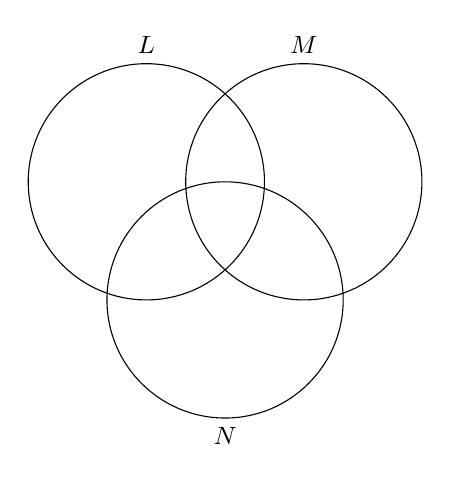
\begin{tikzpicture}[font=\small]
\draw (0,0)circle (1.5) (0,1.5) node[above] {$L$};
\draw(2,0) circle (1.5) (2,1.5) node [above]  {$M$};
\draw(1,-1.5)circle (1.5) (1,-3) node[below]{$N$};
\end{tikzpicture}

\end{center}
\end{esercizio}

\begin{esercizio}
 \label{ese:7.9}
Dati gli insiemi~$C$ delle lettere della parola ``GIARDINO'' e~$D$ delle lettere della
parola ``ORA'', determina la loro unione aiutandoti con la rappresentazione grafica.
 \end{esercizio}

\subsubsection*{7.4 - Insieme intersezione}
 \begin{esercizio}
 \label{ese:7.10}
Dati~$A=\{\text{1, 2, 4, 5}\}$ e~$B=\{\text{1, 3, 4, 5, 8}\}$ determina la loro
intersezione dopo aver rappresentato gli insiemi mediante diagrammi di
Eulero-Venn.
\end{esercizio}

\begin{esercizio}
 \label{ese:7.11}
Dati gli insiemi~$C$ delle lettere della parola ``LIBRO'' e~$D$ delle lettere della
parola ``PASTA'' determina la loro intersezione aiutandoti con la rappresentazione grafica.
\end{esercizio}

\begin{esercizio}
 \label{ese:7.12}
Considerando i~3 insiemi~$S=\{$a, b, c, e, f, s, t$\}$, $T=\{$a, c, g, h, l, s$\}$ e~$U=\{$b, c, d, g, s, t$\}$,
determina l'insieme intersezione dando sia la rappresentazione grafica sia quella tabulare.
 \end{esercizio}

\begin{esercizio}
 \label{ese:7.13}
 Determina l'intersezione tra i seguenti insiemi:
\begin{enumeratea}
 \item $A=\{-3$, $-2$, $-1$, $0$, $+1$, $+2$, $+3\}$, $B=\{-2$, $-1$, $0$, $+1$, $+2$, $+3$, $+4\}$; $A\cap B=\ldots$
 \item $A=\{x\in\insN\mid 2\le x\le~5\}$, $B=\{x\in\insN\mid 3<x<7\}$; $B\cap A=\ldots$
 \item $A=\{x\in\insZ\mid -5\le x\le+5\}$, $B=\{x\in\insZ\mid -15\le x<3\}$; $A\cap B=\ldots$
 \item $A=\{x\in\insN\mid x>100\}$, $B=\{x\in\insN\mid 10<x<20\}$; $B\cap A=\ldots$
 \item $A=\{l$ una lettera di ``SATURNO''$\}$, $B=\{l$ una lettera di ``NETTUNO''$\}$; $A\cap B=\ldots$
\end{enumeratea}
\end{esercizio}

\subsubsection*{7.5 - Insieme differenza}
\begin{esercizio}
\label{ese:7.14}
Dati gli insiemi~$E=\{x\mid x$ è una lettera della parola ``cartellone''$\}$ e
$F=\{x\mid x$ è una lettera della parola ``martello''$\}$, determina
$E-F$ e~$F-E$.
\end{esercizio}

\subsubsection*{7.5 - Insieme complementare}
\begin{esercizio}
\label{ese:7.15}
Verifica, utilizzando la rappresentazione grafica, che
\begin{multicols}{2}
 \begin{enumeratea}
 \item $\overline{A}_{U}\cup A=U$;
 \item $(A-B)\cup (B-A)\cup (\overline{A\cup B})=\overline{A\cap B}$.
 \end{enumeratea}
\end{multicols}
\end{esercizio}

\begin{esercizio}
 \label{ese:7.16}
Dati~$E$ ed~$F$ sottoinsiemi di un insieme~$U$, l'insieme
definito da~$\overline{E\cap F}$ è uguale a:
\begin{center}
\boxA\quad~$E\cup F$\quad\boxB\quad~$\overline{E\cup F}$\quad\boxC\quad~$E\cap F$\quad\boxD\quad~$\overline{E}\cup\overline{F}$
\end{center}
\end{esercizio}

\begin{esercizio}
 \label{ese:7.17}
Dati~$G$ ed~$H$ sottoinsiemi di un insieme~$U$, l'insieme
definito da~$\overline{G\cup H}$ è uguale a:
\begin{center}
\boxA\quad~$\overline{G\cap H}$\quad\boxB\quad~$\overline{G}\cap\overline{H}$\quad\boxC\quad~$\overline{G\cap \overline{H}}$\quad\boxD\quad nessuno dei precedenti
\end{center}
\end{esercizio}

\subsubsection*{7.6 - Leggi di De Morgan}

\begin{esercizio}
 \label{ese:7.18}
 Dimostra la seconda legge di De Morgan, annerendo gli spazi opportuni.
 \begin{center}
 %\usetikzlibrary{decorations.markings}
%\usetikzlibrary{matrix,fit}
%\usetikzlibrary{positioning}
%\usetikzlibrary{shapes.geometric}
%\usetikzlibrary{decorations.pathreplacing}
%\usetikzlibrary{decorations.text}
%\usetikzlibrary{mindmap}
%\usetikzlibrary{plotmarks}
%\usetikzlibrary{backgrounds}
%\usetikzlibrary{patterns}

% (c) 2012 Dimitrios Vrettos - d.vrettos@gmail.com

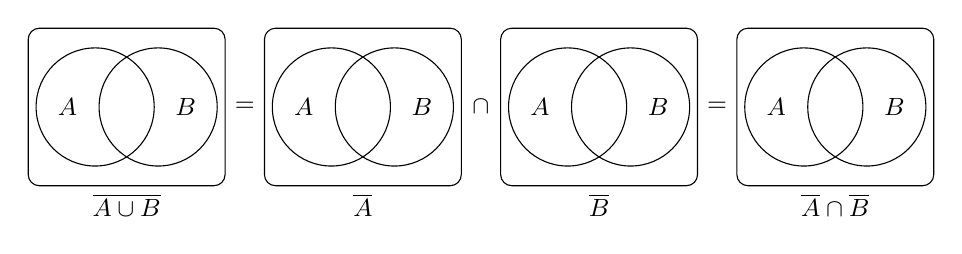
\begin{tikzpicture}[x=5mm,y=5mm,font=\small, outline/.style={draw=circle edge}]
\definecolor{circle area}{gray}{0.9}
\definecolor{circle edge}{rgb}{0,0,0}

\def\firstcircle{(1.7,2) circle (1.5)}
\def\secondcircle{(3.3,2) circle (1.5)}

\begin{scope}[rounded corners]
\foreach \i in {0,6,12,18}
\draw[fill=white] (\i,0) rectangle (\i+5,4);
\end{scope}

\begin{scope}]
\begin{scope}
\clip \firstcircle;
\fill[white] \secondcircle;
\end{scope}
\draw[outline] \firstcircle;
\draw[outline] \secondcircle;
\end{scope}

\begin{scope}[xshift=30mm]
\begin{scope}
\clip \firstcircle;
\fill[white] \firstcircle;
\end{scope}
 \draw[outline]  \firstcircle;
\draw[outline] \secondcircle;
\end{scope}

\begin{scope}[xshift=60mm]
\begin{scope}
\clip \secondcircle;
\fill[white] \secondcircle;
\end{scope}
 \draw[outline]  \firstcircle;
\draw[outline] \secondcircle;
\end{scope}

\begin{scope}[xshift=90mm]
\begin{scope}
\clip \firstcircle;
\fill[white] \secondcircle;
\end{scope}
\draw[outline] \firstcircle;
 \draw[outline] \secondcircle;
\end{scope}

\foreach \x/\xtext in {5.5/$=$,11.5/$\cap$,17.5/$=$}
	\node  at (\x,2) {\xtext};

\foreach \y in {1,7,13,19}
\node  at (\y,2) {$A$};

\foreach \z in {4,10,16,22}
\node  at (\z,2) {$B$};

\foreach \j/\jtext in {2.5/\overline{A\cup B},8.5/\overline{A},14.5/\overline{B},20.5/\overline{A}\cap\overline{B}
}
\node  at (\j,-.5) {$\jtext$};
\end{tikzpicture}



 \end{center}
\end{esercizio}

\subsubsection*{7.7 - Prodotto cartesiano fra insiemi}

\begin{esercizio}
\label{ese:7.19}
Sia~$E=\{x\in\insN\mid 1\le x<3\}$, $F=\{x\mid x$ è una vocale della parola ``TELEFONO''$\}$ e~$G=\{x\in\insN\mid x<-6\}$. Allora:
\begin{enumeratea}
 \item $E=\{1\text{, }\dotfill\}$;
 \item $F=\{\text{e, }\dotfill\}$;
 \item $G=\{\dotfill\}$;
 \item $E\times F=\{(1;\text{e})\text{, }\dotfill\}$;
 \item $F\times E=\{(\text{e};1)\text{, }\dotfill\}$;
 \item $F\times G=\{\dotfill\}$;
 \item $G\times E=\{\dotfill\}$.
\end{enumeratea}
\end{esercizio}

\begin{esercizio}
 \label{ese:7.20}
Quanti sono gli elementi del prodotto cartesiano~$A\times B$, dove~$A$ ha~6 elementi, $B$ ne ha~3:
\begin{center}
 \boxA\quad~9 \quad\boxB\quad~18 \quad\boxC\quad~6 \quad\boxD\quad Non si può sapere.
\end{center}

%\boxA\quad~9 \quad\boxB\quad~18 \quad\boxC\quad~6 \quad\boxD\quad Non si può sapere.
\end{esercizio}


\begin{esercizio}
 \label{ese:7.21}
Sapendo che~$E\times F=\{(\text{x};\text{x})\text{, }(\text{x};\text{y})\text{, }(\text{x};\text{z})\text{, }(\text{y};\text{x})\text{, }(\text{y};\text{y})\text{, }(\text{y};\text{z})\}$, indica gli elementi di~$E$ e di~$F$:
\begin{multicols}{2}
\begin{enumeratea}
 \item $E=\{\dotfill\}$;
 \item $F=\{\dotfill\}$.
\end{enumeratea}
\end{multicols}
\end{esercizio}

\begin{esercizio}
 \label{ese:7.22}
Se~$A\times B$ ha~5 elementi, da quanti elementi possono essere costituiti~$A$ e~$B$?
\begin{center}
 \boxA\quad~1; 5 \quad\boxB\quad~3; 2 \quad\boxC\quad~6; 1 \quad\boxD\quad~2; 3.
\end{center}
\end{esercizio}

\begin{esercizio}
 \label{ese:7.23}
Dati gli insiemi~$A=\{\text{3, 5, 6}\}$ e~$B=\{-2\text{, }1\}$ costruisci il
diagramma cartesiano di~$A\times B$ ed elencane gli elementi.
\end{esercizio}

\begin{esercizio}
 \label{ese:7.24}
 Dato~$A=\{\text{0, 1, 2}\}$ calcola~$A\times A$.
\end{esercizio}

\subsubsection*{7.8 - I diagrammi di Eulero-Venn come modello di un problema}

\begin{esercizio}
\label{ese:7.25}
La scuola ``Step'' organizza corsi di Salsa, Hip Hop e Break Dance.

\begin{enumeratea}
\item Gli iscritti ai corsi sono in tutto~98;
\item 6 frequentano tutti e tre i corsi;
\item 37 frequentano il corso di Salsa;
\item 15 solo i corsi di Salsa e di Hip Hop;
\item 7 solo i corsi Salsa e Break Dance;
\item 9 almeno Hip Hop e Break Dance;
\item 28 Salsa o Break Dance ma non Hip Hop.
\end{enumeratea}

Quanti praticano solo Hip Hop?

Rappresentiamo la situazione con un diagramma di Eulero-Venn.
\begin{center}
 % (c) 2012 Dimitrios Vrettos - d.vrettos@gmail.com
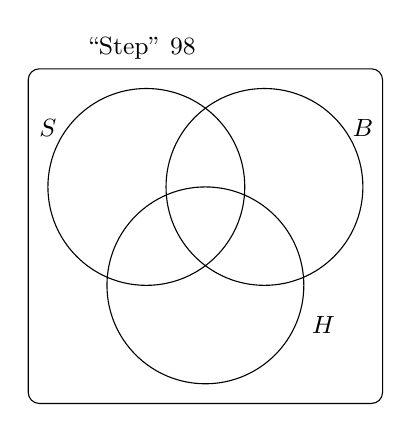
\begin{tikzpicture}[x=5mm, y=5mm,font=\small]

\draw[rounded corners] (0,-5.5) rectangle (9,3) (4.5,3)node[above, anchor=south east] {``Step'' 98};

\draw(3,0) circle (2.5);
\draw(6,0) circle (2.5);
\draw(4.5,-2.5) circle (2.5);

\node at (.5,1.5) {$S$};
\node at (8.5,1.5) {$B$};
\node at (7.5,-3.5) {$H$};

\end{tikzpicture}

\end{center}
$S$ è l'insieme degli iscritti al corso di Salsa, $B$ l'insieme degli iscritti al corso di
Break Dance, $H$ l'insieme degli iscritti al corso di Hip Hop.
\end{esercizio}

\begin{esercizio}
\label{ese:7.26}
Il club ``Argento vivo'' ha~$\np{2500}$ iscritti; nel mese di gennaio ha organizzato alcune
manifestazioni sportive alle quali hanno partecipato~850 degli iscritti
e alcuni tornei di scacchi ai quali hanno partecipato in~780. 320
iscritti al club hanno potuto partecipare, grazie alla perfetta
organizzazione, sia alle manifestazioni sportive sia ai tornei di
scacchi. Quanti soci del club non hanno partecipato a nessuna delle
iniziative e quanti invece hanno partecipato ad almeno una?
\end{esercizio}

\begin{esercizio}[\Ast]
 \label{ese:7.27}
In una scuola di musica si tengono~4 corsi di cui quello di pianoforte è obbligatorio
per tutti i~100 studenti iscritti, mentre quelli di violino, flauto e
chitarra sono facoltativi. Per essere ammessi agli esami di fine anno
bisogna frequentare almeno un corso oltre a quello di pianoforte. Se gli alunni:

\begin{enumeratea}
 \item che frequentano il corso di flauto sono~25 e non frequentano né quello di violino, né quello di chitarra;
 \item iscritti sia al corso di violino sia a quello di chitarra sono~20;
 \item che frequentano il corso di violino sono~46;
 \item che frequentano solo il corso di violino sono tanti quanti quelli che frequentano solo il corso di chitarra.
\end{enumeratea}

Quanti alunni non possono sostenere l'esame finale?
Quale dei seguenti diagrammi di Eulero-Venn può essere preso come modello della situazione?
\begin{center}
 % (c) 2012 Dimitrios Vrettos - d.vrettos@gmail.com

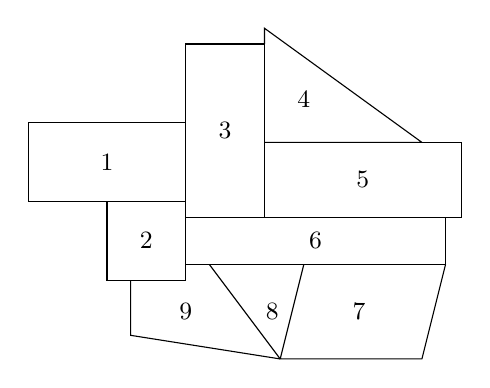
\begin{tikzpicture}[x=10mm,y=10mm, font=\small]
\draw (0,0) rectangle  (2,1) node[midway] {1};
\draw (1,-1) rectangle  (2,0) node[midway] {2};
\draw (2,-.2) rectangle  (3,2) node[midway] {3};
\draw (3,2)-- (3,2.2) -- (5,.75) --(3,.75);
\draw (3,.75) rectangle  (5.5,-.2) node[midway] {5};
\draw (2,-.2) rectangle  (5.3,-.8) node[midway] {6};
\draw (5.3,-.8) -- (5,-2) --(3.2,-2) --(3.5,-.8);
\draw (3.2,-2) -- (2.3,-.8);
\draw (3.2,-2) -- (1.3,-1.7)-- (1.3,-1);
 \node at (3.5,1.3) {4};
 \node at (4.2,-1.4) {7};
 \node at (3.1,-1.4) {8};
 \node at (2,-1.4) {9};
\end{tikzpicture}
\end{center}

\end{esercizio}
\begin{multicols}{2}
\begin{esercizio}[\Ast]
\label{ese:7.28}
I componenti di una compagnia teatrale sanno almeno cantare, ballare,
recitare. Al termine di una rappresentazione si sa che~12 hanno almeno
ballato, 8 hanno almeno cantato e~16 hanno almeno recitato. La
versatilità dei componenti ha permesso che~5 abbiano almeno ballato e
cantato, 3 abbiano almeno cantato e recitato, 8 abbiano ballato e
recitato, 2 ballerini hanno ballato, cantato e recitato. Quanti sono i
componenti della compagnia?
\end{esercizio}

\begin{esercizio}[\Ast]
\label{ese:7.29}
Da un'indagine condotta su consumatori adulti è
risultato che~605 bevono almeno vino, 582 bevono almeno latte, 348
bevono almeno birra, 140 bevono almeno vino e birra, 85 bevono almeno
vino e latte, 56 bevono almeno latte e birra, 25 bevono tutte e tre le
bevande mentre~71 non bevono alcuna delle bevande citate.
\begin{enumeratea}
\item Quante persone bevono una sola bevanda?
\item quante bevono almeno una bevanda?
\item quante sono le persone intervistate?
\end{enumeratea}
\end{esercizio}

\begin{esercizio}[\Ast]
\label{ese:7.30}
In una scuola di lingue sono iscritti~164 studenti; 80 seguono il
corso di francese e~120 il corso di tedesco. Quanti studenti seguono
entrambi i corsi? Quanti studenti seguono
solo il corso di tedesco?
\end{esercizio}

\begin{esercizio}
\label{ese:7.31}
In un classe di~28 allievi, 18 frequentano il laboratorio di teatro,
22 il laboratorio di fotografia, 3 non frequentano alcun laboratorio.
Rappresenta la situazione con un diagramma di Eulero-Venn. Quanto
allievi frequentano entrambi i laboratori? Quanti frequentano almeno un
laboratorio? Quanti non frequentano il laboratorio di teatro?
\end{esercizio}


\begin{esercizio}
\label{ese:7.32}
In una pizzeria, domenica sera, erano presenti~140 persone: 50 hanno
mangiato pizza e calzone, 20 hanno mangiato solo calzone e~15 non hanno
mangiato né pizza né calzone. Il pizzaiolo si chiede se può
conoscere in base alle precedenti informazioni, quante pizze ha
preparato. Aiutalo a risolvere il suo problema illustrando la
situazione con un diagramma di Eulero-Venn, assegnando a ciascun insieme la
sua cardinalità.
\end{esercizio}


\begin{esercizio}
\label{ese:7.33}
In un paese di~$\np{3200}$ abitanti arrivano due quotidiani: il primo è letto da~850
persone, il secondo da~780. Poiché~320 persone leggono entrambi i
quotidiani, quante persone non leggono alcun quotidiano e quante almeno uno?
\end{esercizio}

\begin{esercizio}[Test di ammissione ad Architettura~2008]
\label{ese:7.34}
Nella classe di Asdrubale ci sono~37 allievi. Tutti si sono iscritti
ad almeno una delle due attività extracurriculari (musica e
pallavolo). Alla fine~15 fanno musica e~28 fanno pallavolo.
Quanti allievi, frequentando entrambe le attività, hanno la
necessità di programmare gli orari per evitare sovrapposizioni?
\begin{center}
 \boxA~13\quad\boxB~9\quad\boxC~16\quad\boxD~22\quad\boxE~6
\end{center}
\end{esercizio}



\begin{esercizio}[Test di ammissione a Medicina~2008]
\label{ese:7.35}
In un'aula scolastica, durante la ricreazione, 14
studenti stanno seduti, 8 mangiano la pizza. Con questi dati si può
concludere con certezza che il numero totale~$N$ degli studenti è:
\begin{center}
 \boxA\quad~$N>14$\quad\boxB\quad~$N<14$\quad\boxC\quad~$N>22$\quad\boxD\quad~$N = 22$\quad\boxE\quad~$N\ge~14$
\end{center}
\end{esercizio}


\begin{esercizio}
\label{ese:7.36}
In una scuola di~150 alunni ci sono~23 studenti che frequentano il corso ECDL, 41 studenti che frequentano solo il corso di Inglese, 3
studenti che frequentano tutti e due i corsi. Quanti sono gli studenti che frequentano solo il corso ECDL? Quanti studenti non frequentano
nessuno dei due corsi?
\end{esercizio}

\begin{esercizio}
\label{ese:7.37}
In un giorno di vacanza, 20 alunni dovrebbero studiare latino e
matematica per recuperare le lacune: 8 non studiano latino, 10 studiano
matematica e~4 non studiano niente. Quanti alunni studiano entrambe le
materie?
\end{esercizio}

\begin{esercizio}
\label{ese:7.38}
In una classe di~20 alunni si sta organizzando una gita
scolastica. Durante l'assemblea gli alunni raccolgono
informazioni sulle mete già visitate: 18 hanno visitato Venezia, 14
Roma, 5 Firenze. Solo~3 hanno visitato tutte e tre le città, 5 hanno
visitato Firenze e Venezia, 3 solo Venezia. Quanti hanno visitato solo
Firenze? Quanti hanno visitato Firenze e Roma? Quanti non hanno
visitato nessuna delle tre città? Quanti non hanno visitato Roma?
\end{esercizio}
\end{multicols}
\subsection{Esercizi riepilogativi}

\begin{esercizio}
Siano~$A=\{x\in\insN\mid 1\le x\le~15\}$ e~$B=\{x\in\insN\mid 2\le x\le 20\}$.
\begin{center}
% (c) 2012 Dimitrios Vrettos - d.vrettos@gmail.com
\begin{tikzpicture}[x=3mm, y=5mm,font=\small]

\draw[->, thick] (-1,0)--(24,0) node [above left] {$\insN$};
\draw[pattern =north east lines, pattern color=RedOrange] (1,0) rectangle (15,1) (1,1)node[left] {$A$};
\draw[pattern =north west lines, pattern color=CornflowerBlue] (2,0) rectangle (20,1.5) node[right]{$B$};

\foreach \x/\xtext in {1/1,2/2,15/15,20/20}
\draw[fill] (\x,0)circle (1pt) (\x,0)node [below]{\xtext};
\end{tikzpicture}

\end{center}
Quale delle seguenti affermazioni è vera:
\begin{center}
\boxA\quad~$A\subset B$\quad\boxB\quad~$B\supset A$\quad\boxC\quad$A=B$\quad\boxD\quad$B\not\subset A$
\end{center}
\end{esercizio}

\begin{esercizio}
 Siano~$A=\{x\in\insN\mid x$ è pari e $(1\le x\le 20)\}$ e~$B=\{x\in\insN\mid x$ è multiplo di~6 e $2\le x\le 18\}$.
Quale affermazione è vera?
\begin{center}
 \boxA\quad~$A\subset B$\quad\boxB\quad~$B\supset A$\quad\boxC\quad~$A=B$\quad\boxD\quad~$B\subset A$
\end{center}
\end{esercizio}

\begin{esercizio}
Siano~$A=\{x\in\insN\mid 3\le x\le 10\}$ e~$B=\{x\in\insN\mid 2\le x\le 20\}$.
Quali delle seguenti affermazioni è vera:
\begin{center}
 \boxA\quad~$A\subset B$\quad\boxB\quad~$B\supset A$\quad\boxC\quad~$A=B$\quad\boxD\quad~$B\not\subset A$
\end{center}
\end{esercizio}

\begin{esercizio}
Individua tutti i possibili sottoinsiemi propri formati da tre elementi dell'insieme~$C=\{$a, e, i, o, u$\}$.
\end{esercizio}

\begin{esercizio}
Sia~$A=\{$1, 2, 3, 4$\}$ scrivi i possibili sottoinsiemi propri e impropri di~$A$.
\end{esercizio}

\begin{esercizio}
Associa a ogni diagramma la corretta rappresentazione grafica (ci può essere più di una risposta corretta).

\TabPositions{5cm}
\begin{enumeratea}
 \item $M\subset P$ \tab\boxA\quad\boxB\quad\boxC\quad\boxD\quad\boxE
\item $P\supseteq M$ \tab\boxA\quad\boxB\quad\boxC\quad\boxD\quad\boxE
\item $M\subseteq (M\cup P)$ \tab\boxA\quad\boxB\quad\boxC\quad\boxD\quad\boxE
\item $M\not\subset P$ \tab\boxA\quad\boxB\quad\boxC\quad\boxD\quad\boxE
\item $P\subset (P\cup M)$ \tab\boxA\quad\boxB\quad\boxC\quad\boxD\quad\boxE
\item $M\neq P$ \tab\boxA\quad\boxB\quad\boxC\quad\boxD\quad\boxE
\end{enumeratea}
\begin{center}
% (c) 2012 Dimitrios Vrettos - d.vrettos@gmail.com
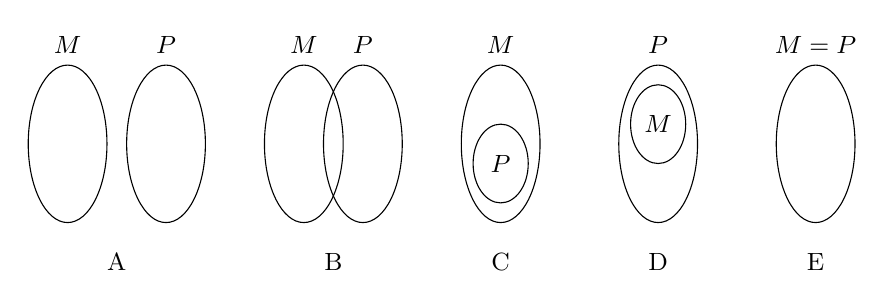
\begin{tikzpicture}[x=5mm, y=5mm,font=\small]

\draw (0,0) ellipse (1 and 2) (0,2.5)node {$M$};
\draw (2.5,0) ellipse (1 and 2)(2.5,2.5) node {$P$};
\node  at (1.25,-3) {A};

\begin{scope}[xshift=30mm]
\draw (0,0) ellipse (1 and 2) (0,2.5)node {$M$};
\draw (1.5,0) ellipse (1 and 2)(1.5,2.5) node {$P$};
\node  at (.75,-3) {B};
\end{scope}

\begin{scope}[xshift=55mm]
\draw (0,0) ellipse (1 and 2) (0,2.5)node {$M$};
\draw (0,-.5) ellipse (.7 and 1) node {$P$};
\node  at (0,-3) {C};
\end{scope}

\begin{scope}[xshift=75mm]
\draw (0,0) ellipse (1 and 2) (0,2.5)node {$P$};
\draw (0,.5) ellipse (.7 and 1) node {$M$};
\node  at (0,-3) {D};
\end{scope}

\begin{scope}[xshift=95mm]
\draw (0,0) ellipse (1 and 2) (0,2.5)node {$M=P$};
\node  at (0,-3) {E};
\end{scope}
\end{tikzpicture}

\end{center}
\end{esercizio}
%\newpage
\begin{esercizio}
Determina l'unione tra i seguenti insiemi:

\begin{enumeratea}
 \item $A=\{-3$, $-2$, $-1$, $0$, $+1$, $+2$, $+3\}$, $B=\{-2$, $-1$, $0$, $+1$, $+2$, $+3$, $+4\}$. $A\cup B=\dotfill$;
 \item $A=\{x\in\insN\mid 2\le x\le 5\}$, $B=\{x\in\insN\mid 3<x<7\}$. $A\cup B=\dotfill$;
 \item $A=\{x\in\insZ\mid -5\le x\le +5\}$, $B=\{x\in\insZ\mid -15\le x<3\}$. $A\cup B=\dotfill$;
 \item $A=\{x\in\insN\mid x>100\}$, $B=\{x\in\insN\mid 10<x<20\}$. $A\cup B=\dotfill$;
 \item $A=\{l$ è una lettera di ``SATURNO''$\}$, $B=\{l$ è una lettera di ``NETTUNO''$\}$. $A\cup B=\dotfill$.
\end{enumeratea}
\end{esercizio}

\begin{esercizio}
Sia~$M_{3}$ l'insieme dei multipli~3 e~$M_{4}$ l'insieme dei multipli di~4, in
generale~$M_{n}$ l'insieme dei multipli del numero~$n$.

 \begin{enumeratea}
 \item Calcola~$M_{3}\cap M_{4}$. Si tratta di~$M\ldots$ l'insieme dei multipli di \ldots;
 \item calcola~$M_{6}\cap M_{4}$. Si tratta di~$M\ldots$ l'insieme dei multipli di \ldots;
 \item calcola~$M_{60}\cap M_{48}$ \ldots;
 \item sai dedurre una regola che, dati due numeri naturali~$m$ e~$n$ calcoli~$M_{m}\cap M_{n}$? Può accadere che questo insieme sia vuoto?
 \end{enumeratea}
\end{esercizio}


\begin{esercizio}
Sia~$D_{4}$ l'insieme dei divisori di~4 e~$D_{6}$ l'insieme dei divisori di~6, in
generale~$D_{n}$ l'insieme dei divisori del numero~$n$.

\begin{enumeratea}
 \item Calcola~$D_{4}\cap D_{6}$. Si tratta di~$D\ldots$ l'insieme dei divisori di \ldots;
 \item calcola~$D_{60}\cap D_{48}$ \ldots;
 \item sai dedurre una regola che, dati due numeri naturali~$m$ e~$n$,
calcoli~$D_{m}\cap D_{n}$? Può accadere che questo insieme sia
vuoto? Qual è il numero minimo di elementi che può contenere?
\end{enumeratea}
\end{esercizio}

\begin{esercizio}
$A=\{x\mid x\in\insQ,0<x<\frac{3}{2}\}$ e~$B=\{x\mid x\in\insQ\text{, }1<x<6\}$, calcola~$A\cap B=\ldots$
\end{esercizio}

\begin{esercizio}
$A=\{x\mid x\in\insQ,-1<x<0\}$ e~$B=\{x\mid x\in\insQ\text{, }\frac{1}{3}<x<6\}$, calcola~$A\cap B=\ldots$
\end{esercizio}

\begin{esercizio}
$A=\{x\mid x\in\insQ,-5<x<10\}$ e~$B=\{x\mid x\in\insQ\text{, }\frac{1}{3}<x<6\}$, calcola~$A\cap B=\ldots$
\end{esercizio}

\begin{esercizio}
$A=\{x\mid x\in\insQ,0\le x<10\}$ e~$B=\{x\mid x\in\insQ\text{, }\frac{1}{3}<x\le~6\}$, calcola~$A\cap B=\ldots$
\end{esercizio}

\begin{esercizio}
Dato l'insieme~$A=\{$3, 4, 5, 6, 7, 8, 9, 12, 32$\}$ e il suo sottoinsieme~$B$ dei multipli di~3, determina gli
insiemi~$A-B$ e~$B-A$.
\end{esercizio}

\begin{esercizio}
Dato l'insieme~$X=\{x\in\insN\mid 10\le x\le~100\}$ e~$Y=\{y\in\insN\mid 10<y<100\}$ determina~$X-Y$ e~$Y-X$.
\end{esercizio}

\begin{esercizio}
Determina la differenza tra i seguenti insiemi:

\begin{esercizio}
Dati gli insiemi~$C$ e~$D$ tali che~$C\subset D$
completa le seguenti relazioni aiutandoti con la rappresentazione
grafica:
\begin{multicols}{3}
\begin{enumeratea}
\item $D-C=\ldots$;
\item $D\cap \overline{C}=\ldots$;
\item $\overline{C\cap D}=\ldots$;
\item $C\cup \overline{C}=\ldots$;
\item $C-D=\ldots$;
\item $C\cap \overline{C}=\ldots$
\end{enumeratea}
\end{multicols}
\end{esercizio}

\begin{enumeratea}
\item $A=\{-3$, $-2$, $-1$, $0$, $+1$, $+2$, $+3\}$, $B=\{-2$, $-1$, $0$, $+1$, $+2$, $+3$, $+4\}$. $A-B=\ldots$;
\item $A=\{x\in\insN\mid 2\le x\le~5\}$, $B=\{x\in\insN\mid 3<x<7\}$. $B-A=\ldots$;
\item $A=\{x\in\insZ\mid -5\le x\le +5\}$, $B=\{x\in\insZ\mid -15\le x<3\}$. $A-B=\ldots$;
\item $A=\{x\in\insN\mid x>100\}$, $B=\{x\in\insN\mid 10<x<20\}$. $B-A=\ldots$;
\item $A=\{l$ è una lettera di ``SATURNO''$\}$, $B=\{l$ è una lettera di ``NETTUNO''$\}$. $A-B=\ldots$
\end{enumeratea}
\end{esercizio}
\pagebreak
\begin{esercizio}
Quale delle seguenti scritture corrisponde a~$\overline{{X\cap \overline{Y}}}$:
\begin{multicols}{4}
 \begin{enumeratea}
 \item $\overline{X}\cup \overline{Y}$
 \item $\overline{X}\cap \overline{Y}$
 \item $\overline{X}\cup Y$
 \item $X\cup \overline{Y}$
 \end{enumeratea}
\end{multicols}
\end{esercizio}


\begin{esercizio}
Esegui le operazioni indicate~$A\cup B$, $A\cap B$, $A-B$.

\begin{enumeratea}
\item $A=\{$2, 4, 6, 8$\}$, $B=\{$1, 3, 6, 9$\}$;
\item $A=\{$a, e, i, o, u$\}$, $B=\{$a, b, c, d, e$\}$;
\item $A=\emptyset$, $B=\{0\}$;
\item $A=\{x\in\insN\mid x$ è pari$\}$, $B=\{x\in\insN\mid x$ è dispari$\}$;
\item $A=\{x\in\insN\mid x$ è multiplo di~2$\}$, $B=\{x\in\insN\mid x$ è multiplo di~4$\}$;
\item $A=\{x\in\insZ\mid -5\le x\le~5\}$, $B=\{x\in\insZ\mid -2\le x\le~8\}$;
\item $A=\{x\in\insN\mid x$ è lettera di ``casa''$\}$, $B=\{x\in\insN\mid x$ è lettera di ``caserma''$\}$.
\end{enumeratea}
\end{esercizio}

\begin{esercizio}
Dato~$A=\{x\in\insN\mid x$ è multiplo di~2$\}$ determina~$\complement_{\insN}A$.
\end{esercizio}

\begin{esercizio}
Dato~$A=\{$I, II, III$\}$ e~$B=\{$a, b$\}$ determina~$A\times B$.
\end{esercizio}

\begin{esercizio}
Dato~$B=\{\text{1, 2, 3}\}$ calcola~$(B\cup B)\cap B$.
\end{esercizio}

\begin{esercizio}
Dati $A=\{$2, 4, 6, 8, 10, 12, 14, 16, 18, 20$\}$, $B=\{$3, 6, 9, 12, 15, 18$\}$ e
$C=\{$1, 3, 5, 7, 9, 11, 13, 15, 17, 19$\}$, calcola
$A\cap B$, $A\cup C$, $(A\cap B)\cup C$, $B\cap C$, $(A\cup B)\cap(B\cup C)$.
\end{esercizio}

\begin{esercizio}
Dati $A=\{x\in\insZ\mid -5\le x<2\}$ e $B=\{x\in\insN\mid -3<x\le~2\}$, calcola
$A\cup B$, $A\cap B$, $B-A$, $\complement_{A}B$, $A\times(A\cap B)$ e~$\wp (B-A)$.
\end{esercizio}

\begin{esercizio}
Per ciascuna delle seguenti affermazioni false dai un controesempio.

\begin{enumeratea}
 \item $A\cup B=A$;
\item $A\cap B=\emptyset\:\Rightarrow\:A=\emptyset $;
\item se~$x$ è multiplo di~2 allora è anche multiplo di~4;
\item se~$\card A =2$ e~$\card B = 5$ allora~$\card A\cup B=7$;
\item se~$\card A =2$ e~$\card B = 5$ allora~$\card A\cap B=2$.
\end{enumeratea}
\end{esercizio}

\begin{esercizio}
In base alla figura rispondi alle domande:
\begin{multicols}{2}
\TabPositions{4.5cm}
\begin{enumeratea}
\item L'insieme~$E$ ha~5 elementi \tab\boxV\quad\boxF
\item $2\in E$ \tab\boxV\quad\boxF
\item $3\notin G$ \tab\boxV\quad\boxF
\item $F\subset G$ \tab\boxV\quad\boxF
\item $F\subset E$ \tab\boxV\quad\boxF
\item $\emptyset \subseteq G$ \tab\boxV\quad\boxF
\item $\card(E)=8$ \tab\boxV\quad\boxF
\item $10\in E$ \tab\boxV\quad\boxF
\item $F\cap E=F$ \tab\boxV\quad\boxF
\item $F\cup G=E$ \tab\boxV\quad\boxF
\item $(E-F)-G=\{\text{1, 4}\}$ \tab\boxV\quad\boxF
\end{enumeratea}
\begin{center}
 % (c) 2012 Dimitrios Vrettos - d.vrettos@gmail.com
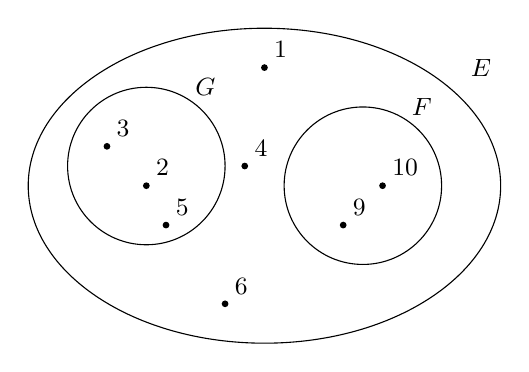
\begin{tikzpicture}[x=5mm, y=5mm,font=\small]

\draw (0,0) ellipse (6 and 4) (5.5,3)node {$E$};
\draw (2.5,0) circle (2)(4,2) node {$F$};
\draw (-3,.5) circle (2)(-1.5,2.5) node {$G$};

\draw[fill](-3,0) circle (1pt ) node[above right]  {2};
\draw[fill](-2.5,-1) circle (1pt ) node[above right]  {5};
\draw[fill](-4,1) circle (1pt ) node[above right]  {3};

\draw[fill](3,0) circle (1pt ) node[above right]  {10};
\draw[fill](2,-1) circle (1pt ) node[above right]  {9};

\draw[fill](0,3) circle (1pt ) node[above right]  {1};
\draw[fill](-.5,.5) circle (1pt ) node[above right]  {4};
\draw[fill](-1,-3) circle (1pt ) node[above right]  {6};
\end{tikzpicture}

\end{center}
\end{multicols}
\end{esercizio}
\pagebreak
\begin{esercizio}
Dato l'insieme~$A=\{$0, 1, 5, 6, 9$\}$ stabilisci
quali dei seguenti sono o meno suoi sottoinsiemi, completando con gli
opportuni simboli le scritture a fianco indicate.
\begin{multicols}{2}
\TabPositions{3cm}
\begin{enumeratea}
\item $B=\{$1, 5, 6$\}$ \tab $B\ldots A$
\item $C=\{$0, 1, 3, 5$\}$ \tab $C \ldots A$
\item $D=\{ \}$ \tab $D \ldots A$
\item $E=\{0\}$ \tab $E \ldots A$
\item $F=\{$5, 6, 7$\}$ \tab $F \ldots A$
\item $G=\{$6, 0, 1, 5, 9$\}$ \tab $G\ldots A$
\end{enumeratea}
\end{multicols}
\end{esercizio}

\begin{esercizio}
Siano dati i seguenti insiemi~$C=\{x\mid x$ è una lettera della parola ``REMARE''\}, $D=\{x\mid x$ è una lettera della parola ``VOLARE''\},
$E=\{x\mid x$ è una lettera della parola ``AMARE''\},
indica quali delle seguenti relazioni sono vere:
\begin{center}
\boxA\quad~$D\subseteq C$\quad\boxB\quad~$D\not\subset E$\quad\boxC\quad~$C=E$\quad\boxD\quad~$E\supseteq C$
\end{center}
\end{esercizio}

\begin{esercizio}
Completa la seguente tabella:

\begin{tabular*}{.9\textwidth}{@{\extracolsep{\fill}}*{2}{cl}}
\toprule
Simbologia & Significato\\
\midrule
$A=\{a\text{, }b\text{, }c\text{, }d\}$ & $A$ è formato dagli \dotfill~$a\text{, }b\text{, }c\text{, }d$.\\
$a\in A$ & L'elemento~$a$ \dotfill all'insieme~$A$.\\
\dotfill & L'elemento f non appartiene all'insieme~$A$.\\
$B\subset A$ & L'insieme~$B$ è \ldots\ldots nell'insieme~$A$, ovvero~$B$ è un \ldots\ldots di~$A$.\\
\dotfill & L'insieme vuoto è un sottoinsieme di~$A$.\\
\dotfill & L'insieme~$C$ è l'unione degli insiemi~$A$ e~$B$.\\
$D=A\cap B$ & L'insieme~$D$ è \dotfill degli insiemi~$A$ e~$B$.\\
$A\cap F=\emptyset $& $A$ e~$F$ sono insiemi \dotfill cioè non hanno \dotfill \\
$L=\complement_{A}B$ & L'insieme~$L$ è \dotfill \\
\dotfill & L'insieme~$M$ è la differenza tra~$A$ e~$B$.\\
\bottomrule
\end{tabular*}
\end{esercizio}

\begin{esercizio}
Rappresenta graficamente l'insieme~$A=\{x\in\insN\mid x\le 25$ e $x$ è pari$\}$ e
$B=\{x\in\insN\mid x\le 27$ e $x$ è multiplo di~4$\}$ e stabilisci se~$A\supseteq B$.
\end{esercizio}

\begin{esercizio}
Verifica usando i diagrammi di Eulero-Venn che se~$A\subset B$ e~$B\subset C$ allora~$A\subset C$. Le relazioni valgono
anche se il simbolo~``${\subset}''$ viene sostituito con~``${\subseteq}''$?
\end{esercizio}

\begin{esercizio}
Dato~$A=\{\text{do, re, mi}\}$ determina l'insieme delle parti~$\wp (A)$.
\end{esercizio}

\begin{esercizio}
Considerato l'insieme~$X=\{\text{a, c, d, t, o}\}$ stabilisci se le seguenti affermazioni sono vere o false.

\TabPositions{8cm}
\begin{enumeratea}
\item $\{x\mid x\text{ è una vocale della parola ``carota''}\} \subset X$ \tab\boxV\quad\boxF
\item $\{\text{a, t}\}\not\subset \wp (X)$ \tab\boxV\quad\boxF
\item $\{\text{a, t}\}\in \wp (X)$ \tab\boxV\quad\boxF
\item $0\in X$ \tab\boxV\quad\boxF
\item $\emptyset \in \wp (X)$ \tab\boxV\quad\boxF
\item $X\in \wp (X)$ \tab\boxV\quad\boxF
\end{enumeratea}
\end{esercizio}

\pagebreak
\begin{esercizio}
Se~$U$ è l'insieme universo degli italiani, $D$ l'insieme delle donne italiane,
$L$ l'insieme degli italiani laureati, $S$ l'insieme degli italiani sposati, cosa rappresentano
i seguenti insiemi?
\begin{multicols}{3}
\begin{enumeratea}
\item $\overline{D}$;
\item $L\cap D$;
\item $\overline{{L\cup D\cup S}}$;
\item $L-S$;
\item $\overline{{L}}\cap S$;
\item $\overline{{L\cap D\cap S}}$.
\end{enumeratea}
\end{multicols}
\end{esercizio}


\begin{esercizio}
Quanti elementi ha~$\wp (H)$ sapendo che $H$ ha~7 elementi?
\begin{center}
 \boxA\quad~49\quad\boxB\quad~64\quad\boxC\quad~128\quad\boxD\quad~7\quad\boxE\quad14
\end{center}
\end{esercizio}

\begin{esercizio}
Scrivi l'insieme che ha per insieme delle parti:
$\{\emptyset\text{, }\{\text{Mauro}\}\text{, }\{\text{Mario}\}\text{, }\{\text{Mauro, Mario}\}\}$.
\end{esercizio}

\begin{esercizio}
Se~$A\cup B=B$ cosa puoi dire di~$A$ e~$B$?
\begin{center}
 \boxA\quad~$B\subseteq A$\quad\boxB\quad~$A\notin B$\quad\boxC\quad~$A\subseteq B$\quad\boxD\quad~$A\subset B$\quad\boxE\quad$A\cap B=\emptyset $
\end{center}
\end{esercizio}

\begin{esercizio}
Dati gli insiemi~$A=\{\text{10, 20, 30, 40, 50}\}$ e $B=\{\text{20, 30, 50}\}$,
determina un insieme~$C$ tale che:
\begin{multicols}{4}
\begin{enumeratea}
 \item $B\cup C=A$;
 \item $A\cap C=B$;
 \item $C\cup C=B$;
 \item $C\cap C=A$.
\end{enumeratea}
\end{multicols}
\end{esercizio}

\begin{esercizio}
Dati gli insiemi~$A=\{x\in\insN\mid x\le 10$ e $x$ è pari$\}$,
$B=\{x\in\insN\mid x\le 20$ e $x$ è divisibile per~4$\}$ e
$C=\{$1, 2$\}$, determina~$(A\cap B)\times C$.
\end{esercizio}

\begin{esercizio}
Dimostra la proprietà distributiva dell'intersezione rispetto l'unione annerendo gli spazi opportuni.
\begin{center}
 % (c) 2012 Dimitrios Vrettos - d.vrettos@gmail.com
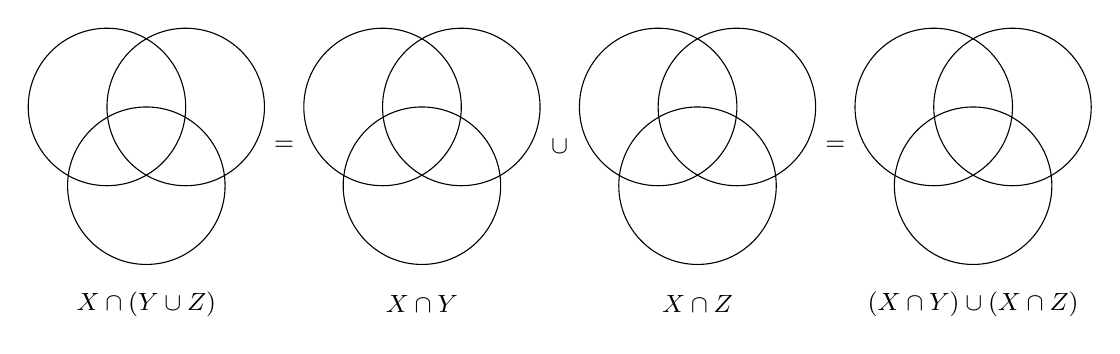
\begin{tikzpicture}[x=5mm, y=5mm,font=\small]

\draw (0,0) circle (2);
\draw (2,0) circle (2);
\draw (1,-2) circle (2);

\begin{scope}[xshift=35mm]
\draw (0,0) circle (2);
\draw (2,0) circle (2);
\draw (1,-2) circle (2);
\end{scope}

\begin{scope}[xshift=70mm]
\draw (0,0) circle (2);
\draw (2,0) circle (2);
\draw (1,-2) circle (2);
\end{scope}

\begin{scope}[xshift=105mm]
\draw (0,0) circle (2);
\draw (2,0) circle (2);
\draw (1,-2) circle (2);
\end{scope}

\foreach \x/\xtext in {4.5/=,11.5/\cup,18.5/=}
\node  at (\x,-1) {$\xtext$};

\foreach \xi/\xitext in {1/$X\cap(Y\cup Z)$,8/$X\cap Y$,15/$X\cap Z$,22/$(X\cap Y)\cup(X\cap Z)$}
\node  at (\xi,-5) {\xitext};
\end{tikzpicture}

\end{center}

\end{esercizio}

\begin{esercizio}
Se~$E-F=E$ cosa puoi dire di~$E$ e~$F$?
\begin{center}
 \boxA\quad~$E\cup F=E$\quad\boxB\quad~$E=F$\quad\boxC\quad~$E\subseteq F$\quad\boxD\quad~$F\subset E$\quad\boxE\quad~$E\cap F=\emptyset $
\end{center}
\end{esercizio}

\begin{esercizio}
Dimostra la proprietà distributiva dell'unione rispetto l'intersezione annerendo gli spazi opportuni
e inserendo le formule opportune.
\begin{center}
 % (c) 2012 Dimitrios Vrettos - d.vrettos@gmail.com
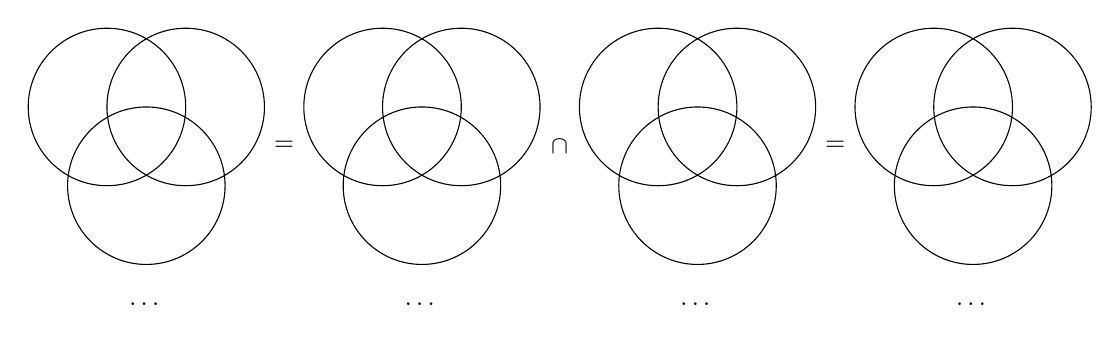
\begin{tikzpicture}[x=5mm, y=5mm,font=\small]

\draw (0,0) circle (2);
\draw (2,0) circle (2);
\draw (1,-2) circle (2);

\begin{scope}[xshift=35mm]
\draw (0,0) circle (2);
\draw (2,0) circle (2);
\draw (1,-2) circle (2);
\end{scope}

\begin{scope}[xshift=70mm]
\draw (0,0) circle (2);
\draw (2,0) circle (2);
\draw (1,-2) circle (2);
\end{scope}

\begin{scope}[xshift=105mm]
\draw (0,0) circle (2);
\draw (2,0) circle (2);
\draw (1,-2) circle (2);
\end{scope}

\foreach \x/\xtext in {4.5/=,11.5/\cap,18.5/=}
\node  at (\x,-1) {$\xtext$};

\foreach \xi in {1,8,15,22}
\node  at (\xi,-5) {\ldots};
\end{tikzpicture}

\end{center}
\end{esercizio}
%\newpage
\begin{esercizio}
Dati i seguenti insiemi~$A=\{x\in\insN\mid x\le~25\}$, $B=\{x\in\insN\mid 4<x\le~9\}$, $C=\{x\in\insN\mid x<25\}$ e~$D=\{x\in\insN\mid x>7\}$.
Scegli fra i seguenti i loro complementari.
\begin{multicols}{2}
\begin{enumeratea}
\item $E=\{x\in\insN\mid x\ge~25\}$;
\item $F=\{x\in\insN\mid x\le~6\}$;
\item $G=\{x\in\insN\mid x>25\}$;
\item $H=\{x\in\insN\mid x<7\}$;
\item $I=\{x\in\insN\mid x<4\text{ e }x\ge~8\}$;
\item $L=\{x\in\insN\mid x<4\text{ o }x\ge~10\}$;
\item $M=\{x\in\insN\mid x\le~4\text{ e }x\ge~9\}$.
\end{enumeratea}
\end{multicols}
\end{esercizio}

\begin{esercizio}
Quali dei seguenti sono sottoinsiemi dei numeri pari? L'insieme dei

\begin{center}
 \boxA\quad multipli di~4\quad\boxB\quad multipli di~3\quad\boxC\quad multipli di~6\quad\boxD\quad numeri primi
\end{center}
\end{esercizio}

\begin{esercizio}[\Ast]
In una classe di~30 allievi~16 hanno debito in matematica, 20 in
italiano, 10 non hanno avuto nessun debito. Rappresenta la situazione
con un diagramma di Eulero-Venn.

\begin{enumeratea}
\item quanti allievi hanno debito in entrambe le materie;
\item quanti allievi hanno almeno un debito;
\item quanti allievi non hanno debito in italiano;
\item quanti allievi non hanno debito in matematica.
\end{enumeratea}
\end{esercizio}

\begin{esercizio}
Quali dei seguenti insiemi possono essere sottoinsiemi dell'insieme dei quadrilateri?
L'insieme dei:
\begin{multicols}{3}
\begin{enumeratea}
 \item quadrati;
 \item rombi;
 \item trapezi;
 \item triangoli equilateri;
 \item poligoni;
 \item cerchi;
 \item parallelogrammi.
\end{enumeratea}
\end{multicols}
\end{esercizio}


\begin{esercizio}
Dati gli insiemi~$A=\{x\mid x\in\insN$, $x<10\}$, $B=\{x\mid x\in\insN$, $5<x\le 16\}$ e
$C=\{x\mid x\in\insN$, $x\ge~7\}$ determina:
\begin{multicols}{4}
\begin{enumeratea}
\item $A\cup B\cup C$;
\item $A\cap B\cap C$;
\item $(A\cup B)\cap C$;
\item $(B\cap C)\cup A$.
\end{enumeratea}
\end{multicols}
\end{esercizio}


\begin{esercizio}
Dato~$A = \{x\mid x$ è un numero naturale, $x$ è pari e $x>12\}$ determina l'insieme complementare di~$A$.
\end{esercizio}

\begin{esercizio}
Quanti sono i sottoinsiemi dell'insieme che contiene come elemento
l'insieme vuoto?
\end{esercizio}

\begin{esercizio}
Dati $A=\{x\mid x$ è divisore di~12$\}$, $B=\{x\mid x$ è divisore di~6$\}$ e
$C=\{x\mid x$ è divisore di~15$\}$, determina:
\begin{multicols}{4}
 \begin{enumeratea}
 \item $A\cup B$;
 \item $A\cup C$;
 \item $A\cup B\cup C$;
 \item $A\cap B$;
 \item $B\cap C$;
 \item $A\cap C$;
 \item $A\cap B\cap C$;
 \item $A\cap(B\cup C)$.
 \end{enumeratea}
\end{multicols}
\end{esercizio}


\begin{esercizio}
Dato l'insieme~$U=\{x\mid x=2n+1$, $n\in\insN$, $0\le n\le~5\}$:

\begin{enumeratea}
\item rappresenta~$U$ in forma tabulare;
\item costruisci due sottoinsiemi propri~$A$ e~$B$ di~$U$ tali che~$A\cap B=\emptyset $;
\item determina~$A\cup B$ e~$A-B$, dai il risultato con rappresentazione tabulare e mediante diagrammi di
Eulero-Venn.
\end{enumeratea}
\end{esercizio}
\pagebreak
\begin{esercizio}
In base agli insiemi rappresentati con il diagramma di Eulero-Venn nella figura determina gli insiemi richiesti:
\begin{multicols}{2}
\begin{enumeratea}
\item $A\cup B$;
\item $\overline{A\cup B\cup C}$;
\item $A\cap B$;
\item $B\cap C$;
\item $A\cap B\cap C$;
\item $A\cap (B\cup C)$;
\item $A\cup (B\cap C)$;
\item $B\cap \overline{C}$;
\item $(A\cup B)-C$;
\item $B\cap \overline{C}$
\item $C-(A\cap B)$;
\item $\overline{(A\cup B)}-C$.
\end{enumeratea}
\begin{center}
 % (c) 2012 Dimitrios Vrettos - d.vrettos@gmail.com
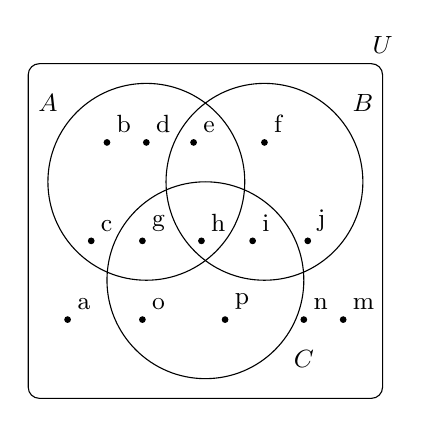
\begin{tikzpicture}[x=5mm, y=5mm,font=\small]

\draw[rounded corners] (-4,-5.5) rectangle (5,3) node[above] {$U$};
\draw (-1,0) circle (2.5) (-3.5,2)node {$A$};
\draw (2,0) circle (2.5) (4.5,2)node {$B$};
\draw (0.5,-2.5) circle (2.5) (3,-4.5)node {$C$};

\foreach \x/\xtext in {-2/b,-1/d,0.2/e,2/f}
\draw[fill] (\x,1)circle(1pt) node[above right]{\xtext};

\foreach \x/\xtext in {-2.4/c,-1.1/g,0.4/h,1.7/i, 3.1/j}
\draw[fill] (\x,-1.5)circle(1pt) node[above right]{\xtext};

\foreach \x/\xtext in {-3/a,-1.1/o,1/p,3/n, 4/m}
\draw[fill] (\x,-3.5)circle(1pt) node[above right]{\xtext};
\end{tikzpicture}

\end{center}
\end{multicols}
\end{esercizio}


\begin{esercizio}
Determina l'insieme~$\wp(A)$, insieme delle parti di~$A$, dove $A$ è l'insieme delle lettere della parola ``NONNA''.
\end{esercizio}

\begin{esercizio}
Nel seguente diagramma di Eulero-Venn gli insiemi~$r$, $s$, $t$
sono rette, gli elementi~$A$, $B$, $C$, $D$ sono punti. Dai una
rappresentazione geometrica, individuando le rette e che corrispondono
alla seguente situazione.

\begin{center}
 % (c) 2012 Dimitrios Vrettos - d.vrettos@gmail.com
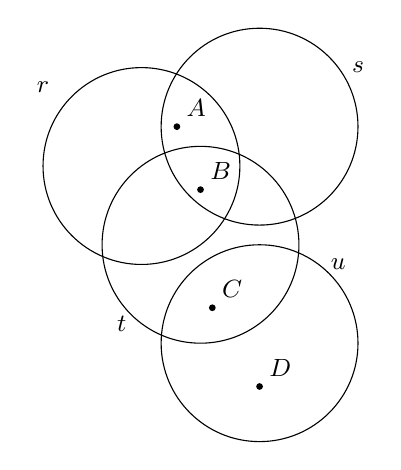
\begin{tikzpicture}[x=5mm, y=5mm,font=\small]
\draw (-1,0) circle (2.5) (-3.5,2)node {$r$};
\draw (2,1) circle (2.5) (4.5,2.5)node {$s$};
\draw (0.5,-2) circle (2.5) (-1.5,-4)node {$t$};
\draw (2,-4.5) circle (2.5) (4,-2.5)node {$u$};

\draw[fill] (-.1,1) circle (1pt) node[above right]  {$A$};
\draw[fill] (.5,-.6) circle (1pt) node[above right]  {$B$};
\draw[fill] (.8,-3.6) circle (1pt) node[above right]  {$C$};
\draw[fill] (2,-5.6) circle (1pt) node[above right]  {$D$};
\end{tikzpicture}

\end{center}
\end{esercizio}

\subsection{Risposte}

\paragraph{7.27.} 3; A.

\paragraph{7.28.} 22.

\paragraph{7.29.} a)~$\np{1048}$,\quad b)~$\np{1279}$,\quad c)~$\np{1350}$.

\paragraph{7.30.} 36; 84.

\paragraph{7.84.} a)~16,\quad b)~20,\quad c)~10,\quad d)~14.


\cleardoublepage
